\section{Overview}

In this thesis so far I have been working in different techniques to help
expand a purely supervised model for Spanish \vsd. The last two chapters
presented two approaches for {\em joint semi-supervised learning}, where the
labeled and unlabeled data (annotated either automatically or manually) are
used together as part of the training data for a supervised classifier (e.g. a
neural network). In this chapter I will cover the last semi-supervised
technique I studied in this thesis.

{\bf Ladder network} is a deep learning model which uses a neural network
architecture to learn both from supervised and unsupervised data presented by
Rasmus et al. \cite{Rasmus:2015aa}. The technique is another example of a
semi-supervised joint learning task. In contrast to self-learning and active
learning, which are wrapper algorithms that use a supervised classifier under
the hood to expand the data from an unlabeled source, ladder networks combine
both datasets in a common {\em objective function} that minimizes using
back-propagation and gradient descent. In the original work, the model was
tested in a machine vision task, but the architecture was general enough to be
able to apply it in the area of Spanish \vsd. 

The key concept behind the construction of a ladder network is to take a
feed-forward neural network (e.g a multilayer perceptron) and treat it as the
encoder part of an autoencoder. Then add a decoder part and use a
reconstruction error calculated layer by layer. The labeled data is used to
minimize the error given by the encoder and a labeled cost function (e.g.
cross-entropy). The unlabeled data traverse the whole autoencoder and the
reconstruction error is minimized. The ladder network cost function is a sum of
both labeled and unlabeled cost functions.

{\em Stacked autoencoders} \cite{Vincent:2010:SDA:1756006.1953039} were a key
idea to help the training of deep neural networks. Using them for {\em
unsupervised pre-training} (also known as {\em fine tuning}), helped deep
neural network architectures converge faster to a solution and avoid the
problem of {\em vanishing gradient} \cite{279181}. Ladder networks draw
inspiration from that idea, but instead of doing the fine tuning of the layers
in the network in a previous step like in unsupervised pre-training, they fine
tune during the training of the network by adding the value of the unsupervised
cost function (of the autoencoder) to the cost function of the feed-forward
neural network. 

This scheme contrasts the one of the wrapper algorithms which uses the purely
labeled cost function of the wrapped classifier. For wrapper algorithms the
unlabeled data adds information by converting an unlabeled instance into a
labeled one. The new information in a ladder network, which comes from the
unlabeled data, is added to the model in a different way. In each epoch the
training algorithm fits the parameters of the network using the whole labeled
dataset (randomly shuffled) but only a portion of the unlabeled dataset. The
unlabeled data adds an extra cost to the train of the networks that avoids it
to overfit the labeled dataset. In the same way, that information helps the
network find a better encoded representation of the unlabeled data that is
useful for the task the ladder network is trying to learn.

I want to assess this particular neural network architecture in the task of
Spanish \vsd~and see how it affects the final performance. The idea is to
tackle the problem of self-learning and its deviation to the most frequent
class. To do that, ladder networks will not start by a supervised model and
then add unlabeled data to it, but rather learn from both the labeled an
unlabeled data in parallel. On the other hand, as the method does not require
human intervention, it overcomes the annotation cost of active learning.

This chapter works on testing the following hypothesis:

\begin{hypothesis}\label{hyp:ladder}
  Ladder networs obtain a better model of the data.
\end{hypothesis}

I expect that the cause for a better model is the integration of unsupervised
data to choose the model that is consistent with the labeled data and at the
same time most adequate to explain the distribution of unlabeled data.

This can be worked through the following subhypotheses:

\begin{subhypothesis}\label{hyp:ladder:1}
  The ladder network model improves over the purely supervised and other
  semi-supervised methods on a held-out test corpus.
\end{subhypothesis}

\begin{subhypothesis}\label{hyp:ladder:2}
  On new annotated examples with this classifier, the representativity of the
  classes is maintained.
\end{subhypothesis}

\begin{subhypothesis}\label{hyp:ladder:3}
  Overfitting of the labeled corpus is avoided by the use of unlabeled data to
  minimize an unsupervised cost function.
\end{subhypothesis}

\begin{itemize}
  \item Experiment \ref{exp:ladder:1} reports the performance of the ladder
    network model over the held-out test set. The performance is measured by
    the F1-score per class. Results shown in Section \ref{sec:ladder:hyp:1}
    serve to accept Hypothesis \ref{hyp:ladder:1}, that the performance over a
    model on held-out test data for the ladder network improves over the
    previous methods.
  \item Experiment \ref{exp:ladder:2} shows the distribution of the classes
    that the model has by automatically annotating instance drawn from an
    unlabeled corpus. This are measured by the proportional count of the
    classes. The results shown in Section \ref{sec:ladder:hyp:2} serve to
    partially accept Hypothesis \ref{hyp:ladder:2} as it is valid for word
    embeddings but not for hand-crafted features.
  \item Experiment \ref{exp:ladder:3} seed the tendency overfitting by
    measuring the error due to variance of a model trained on one dataset over
    other datasets. To measure this I use the learning curve (Metric
    \ref{met:3}) I already explained in previous chapters. It is important to
    note that, this time the learning curve is not measured using the
    information given by labeled data, but it is measured based on the
    information that unlabeled data give to the model. The results of the
    experiments shown in Section \ref{sec:ladder:hyp:3} serve to accept
    Hypothesis \ref{hyp:ladder:3} which states that the use of unlabeled data
    to minimize an unsupervised cost function help to decrease the model
    tendency to overfit. 
\end{itemize}

In Section \ref{sec:ladder:previous} I introduce a brief summary of the ladder
network model, citing the original work and the works from where the authors
draw inspiration to come with this novel approach.

In Section \ref{sec:ladder:methodology} I go through the relevant items that
concern the experimentation in the chapter. Most of the methodology is very
similar to that in previous chapters, I mostly provide pointers to the sections
where this methodology is first described. Section \ref{sec:ladder:model} is
the most important part, where I go through the fine-grained details concerning
the model, including the architecture of the ladder network, the training of
the algorithm and the definition of the cost functions and auxiliary functions.

Section \ref{sec:ladder:results} reports the results of the experiments and
analyzes them in order to accept the stated hypotheses of the chapter.

Finally Section \ref{sec:ladder:conclusions} draws the conclusions of this
chapter, recapitulating the Hypotheses and the implications of accepting or
rejecting them according to the evidence gathered in the results. It ends by
outlining future work.

\section{Relevant work}\label{sec:ladder:previous}

The idea of using unsupervised learning to help training a neural network was
proposed by Suddarth and Kergosien \cite{Suddarth1990}. Most of the methods
that use an auxiliary task to help the supervised learning are only applied at
pre-training, followed by normal supervised learning \cite{Hinton504}. In
contrast, with ladder networks \cite{Rasmus:2015aa} representations are learnt
jointly. Unsupervised learning is implemented through an auxiliary task, for
example, reconstructing the input. In learning, the hidden representations
among supervised and unsupervised tasks are shared, and thus the network
generalizes better. I provide details of the method in what follows.

The Ladder network method presented by Rasmus et al. follows the work by
Valpola \cite{Valpola:2014aa}, who proposed a Ladder network where the
auxiliary task is to denoise representations at every level of the model. The
model structure is an autoencoder with skip connections from the encoder to
decoder and the learning task is similar to that in denoising autoencoders but
applied to every layer, not just the inputs. The skip connections relieve the
pressure to represent details in the higher layers of the model because,
through the skip connections, the decoder can recover any details discarded by
the encoder. Originally, the ladder networks were only applied to unsupervised
learning \cite{Valpola:2014aa,Rasmus:2014aa} but then they were combined with
supervised learning.

The key aspects of ladder networks, as described in \cite{Rasmus:2015aa}, are
the following:

\begin{description}
  \item[Compatibility with supervised methods] The unsupervised part complements
    what is found by supervised learning, adding information while maintaining
    compatibility with the purely supervised model. Furthermore, it can be added
    to existing feed-forward neural networks, for example multilayer perceptrons
    or convolutional neural networks.
  \item[Scalability resulting from local learning] In addition to a supervised
    learning target on the top layer, the model has local unsupervised learning
    targets on every layer, making it suitable for very deep neural networks.
  \item[Computational efficiency] The encoder part of the model corresponds to
    normal supervised learning. Adding a decoder, as proposed in the paper,
    approximately triples the computation during training but not necessarily
    the training time since the same result can be achieved faster through 
    better utilization of the available information. Overall, computation per
    update scales similarly to whichever supervised learning approach is used,
    with a small multiplicative factor.
\end{description}

The steps involved in implementing the Ladder network are typically as follows:
(i) take a feed-forward model which serves for supervised learning as the
encoder; (ii) add a decoder which can invert the mappings on each layer of the
encoder and supports unsupervised learning; and (iii) train the whole Ladder
network by minimizing the sum of all the cost function terms.

\section{Methodology}\label{sec:ladder:methodology}

This chapter explores the use of ladder networks for Spanish \vsd. The model
learns by minimizing a cost function composed of a supervised and an
unsupervised objectives. As it is defined in the original publication, ladder
networks do not add or treat unlabeled data as labeled (unlike self-learning
and active learning). The best comparison possible with the other methods is
done in the held-out test set. However, to have some more reference points I
did some changes over the original scheme in order to make it more comparable
to the self-learning approach.

Once again, the results I show in this chapter try to be as objective as
possible, but there is only a number of possible evaluation metrics and
visualization tools I can use, and some of them may obscure other results.

\subsection{Resources}

As with self-learning, there are two main resources required for ladder
networks: a labeled and an unlabeled dataset. I will keep using the same
datasets I have used through all the thesis: SenSem as supervised data, and
SBWCE as unsupervised data. 

Please refer to Section \ref{sec:supervised:sensem} to see the details of the
SenSem corpus and how it was split intro training/test datasets following a
stratified split application, but retaining at least one example of each class
per split. Like what was done in Chapter \ref{chapter:self-learning}, in the
experiments of this chapter the SenSem dataset was randomly oversampled in the
less frequent classes to have a more uniform distribution of all the classes of
the supervised dataset.

The unlabeled instances are taken from the SBWCE dataset that was described in
Section \ref{sec:embeddings:sbwce} and processed as described in Section
\ref{sec:self-learning:sbwce}. Please refer to those sections for more
information regarding this dataset.

\subsection{Features}

The features used in this part are the same ones used in the previous chapters.
Both hand-crafted features using the hashing trick and word embeddings follow
what has been discussed in all the previous chapters.

For more information on the detail of what are the hand-crafted features used
in this chapter please refer to Section \ref{sec:supervised:features}. For
detailed information on how to deal with the expansion of features given by the
new examples added to the model please refer to Section
\ref{sec:self-learning:handcrafted}.

The word embeddings are the ones trained from the journalistic corpus described
in detail in Section \ref{sec:embeddings:journal}. The method for combining
them into an instance is the concatenation of word vectors described in Section
\ref{sec:embeddings:embeddings}.

\subsection{Ladder network model}\label{sec:ladder:model}

In this section I will explain in more detail the Ladder network model. This is
but a brief introduction following the work presented by Rasmus et al.
\cite{Rasmus:2015aa}. I recommend the reader to refer to their work which
presents a more detailed version of what I describe here.

\subsubsection{Architecture}

The architecture of a ladder network is based on an autoencoder whose encoding
part also works as a supervised classifier and whose decoder part works as an
unsupervised learner by reconstructing the input. The structure of a ladder
network typically follows these steps:

\begin{enumerate}
  \item Set an encoder which works as a supervised classifier using a
    feed-forward model. The network has two encoder paths --clean and
    corrupted. The only difference is that the corrupted encoder adds Gaussian
    noise at all layers. Adding noise serves to avoid overfitting of the
    resulting model.
  \item Set a decoder which works as an unsupervised learner by inverting the
    mappings on each layer of the encoder. The decoder uses a denoising
    function to reconstruct the activations of each layer given the corrupted
    version. The target at each layer is the clean version of the activation
    and the difference between the reconstruction and the clean version serves
    as the denoising cost of that layer.
  \item The supervised cost, that is, the error between the predicted label and
    the ground truth label, is calculated from the output of the corrupted
    encoder and the target label. On the other hand, the unsupervised cost is
    the sum of the denoising cost of all layers scaled by a hyperparameter that
    denotes the importance of each layer. For example, the first layers are
    more important than the last to reconstruct the input. The final cost is
    the sum of the supervised and the unsupervised cost. 
\end{enumerate}

The whole network is trained in a fully-labeled or semi-supervised setting
using standard optimization techniques (such as stochastic gradient descent) to
minimize these costs. Keep in mind the ladder network can work even without
auxiliary unlabeled data, but the original motivation was to make it possible
to take well-performing feed-forward classifiers and augment them with an
auxiliary decoder.

\begin{figure}[ht]
  \centering
  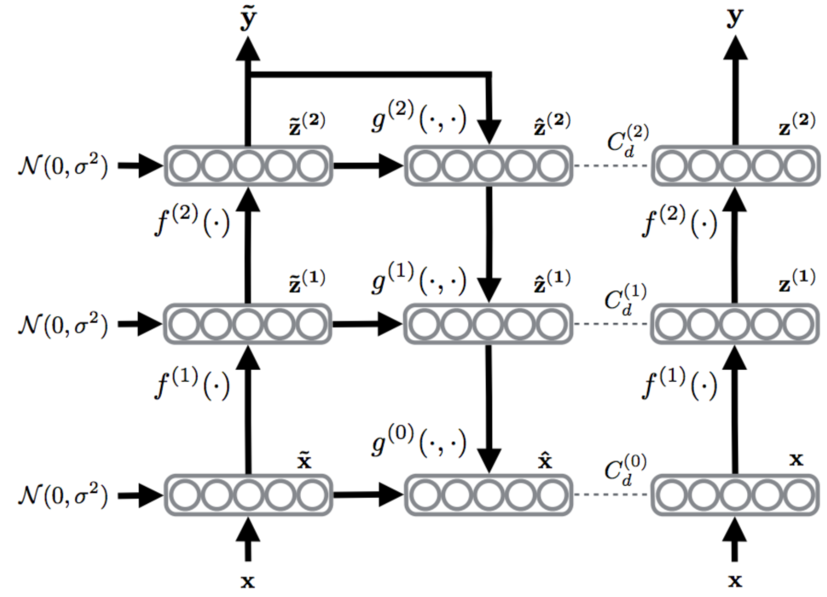
\includegraphics[width=\textwidth]{images/ladder_architecture}
  \caption{
    A conceptual illustration of a ladder network with two hidden layers ($L =
    2$). The feed-forward path ($\mathbf{x} \rightarrow \mathbf{z}^{(1)}
    \rightarrow \mathbf{z}^{(2)} \rightarrow \mathbf{y}$) shares the mappings
    $f^{(l)}$ with the corrupted feed-forward path, or encoder ($\mathbf{x}
    \rightarrow \mathbf{\tilde{z}}^{(1)} \rightarrow \mathbf{\tilde{z}}^{(2)}
    \rightarrow \mathbf{\tilde{y}}$). The decoder ($\mathbf{\hat{z}}^{(2)}
    \rightarrow \mathbf{\hat{z}}^{(1)} \rightarrow \mathbf{\hat{x}}$) consists
    of the denoising functions $g^{(l)}$ and has cost functions $C^{(l)}_{d}$
    on each layer aimed to minimize the difference between
    $\mathbf{\hat{z}}^{(l)}$ and $\mathbf{z}^{(l)}$. The output
    $\mathbf{\tilde{y}}$ of the encoder can also be trained to match available
    labels $t(n)$. Original figure found in the work of Rasmus et al.
    \cite{Rasmus:2015aa}.
  }
  \label{fig:ladder:architecture}
\end{figure}

Figure \ref{fig:ladder:architecture} shows the structure of a ladder network.
The corrupted path (left in the Figure) adds Gaussian noise $\mathcal{N}(0,
\sigma^{2})$ to each layer of the encoder. Every layer contributes to the cost
function, a term $C^{(l)} = ||\mathbf{z}^{(l)} - \mathbf{\hat{z}}^{(l)}||^{2}$
which trains the layers above (both encoder and decoder) to learn the denoising
function $\mathbf{\hat{z}}^{(l)} = g^{(l)}(\mathbf{\tilde{z}}^{(l)},
\mathbf{\hat{z}^{(l+1)}})$ which maps the corrupted $\mathbf{\tilde{z}}^{(l)}$
onto the denoised estimate $\mathbf{\hat{z}}^{(l)}$. As the estimate
$\mathbf{\hat{z}}^{(l)}$ incorporates all prior knowledge about $\mathbf{z}$,
the same cost function term also trains the encoder layers below to find
cleaner features which better match the prior expectation.

Since the cost function needs both the clean $\mathbf{z}^{(l)}$ and corrupted
$\mathbf{\tilde{z}}^{(l)}$, during training the encoder is run twice: a clean
pass for $\mathbf{z}^{(l)}$ and a corrupted pass for
$\mathbf{\tilde{z}}^{(l)}$. 

In denoising autoencoders \cite{Vincent:2010:SDA:1756006.1953039}, an
autoencoder is trained to reconstruct the original observation $\mathbf{x}$
from a corrupted version $\mathbf{\tilde{x}}$. Learning is based simply on
minimizing the norm of the difference of the original $\mathbf{x}$ and its
reconstruction $\mathbf{\hat{x}}$ from the corrupted $\mathbf{\tilde{x}}$; that
is the cost is $||\mathbf{\hat{x}} - \mathbf{x}||^{2}$. The main difference is
that in ladder networks the cost of reconstruction is calculated layer by layer
adding the denoising functions $\mathbf{\hat{z}} = g(\mathbf{z})$.

One way to picture the Ladder network is to consider it as a collection of
nested denoising autoencoders which share parts of the denoising machinery with
each other via the cost function $C_{d}$. If this function were not used, from
the viewpoint of the autoencoder on layer $l$, the representations on the
higher layers would be opaque, treated as hidden neurons. In other words, there
would be no particular reason why intermediate representation
$\mathbf{\hat{z}}^{(l+i)}$ as produced by the decoder should resemble the
corresponding representations $\mathbf{z}^{(l+i)}$ as produced by the encoder.
It is only the cost function $C^{(l+i)}_{d}$ that ties these together and
forces the inference to proceed in reverse order in the decoder. This sharing
helps a deep denoising autoencoder to learn the denoising process as it splits
the task into meaningful sub-tasks of denoising intermediate representations.

Batch normalization \cite{Ioffe:2015aa} is applied to each preactivation
including the topmost layer to improve convergence (due to reduced covariate
shift) and to prevent the denoising cost from encouraging the trivial solution
(encoder outputs constant values as these are the easiest to denoise). Direct
connection between a layer and its decoded reconstruction are used. The network
is called a Ladder network because the resulting encoder/decoder architecture
resembles a ladder because the cost function between mirroring layers could be
seen as the strings in ladder steps.

\subsubsection{Training of the network}

\begin{algorithm}[ht]
  \caption{Calculation of the output and cost function of the Ladder Network.
  Taken from Rasmus et al. \cite{Rasmus:2015aa}}
  \label{alg:ladder}
  \begin{multicols}{2}
  \begin{algorithmic}
    \REQUIRE $\mathbf{x}(n)$
    \STATE \# Corrupted encoder and training output
    \STATE {
      $\mathbf{\tilde{h}}^{(0)} \leftarrow \mathbf{\tilde{z}}^{(0)} \leftarrow
      \mathbf{x}(n) + \mathtt{noise}$
    }
    \FOR{ $l = 1$ \TO $L$ }
      \STATE {
        $\mathbf{\tilde{z}}^{(l)}_{\text{pre}} \leftarrow
        \mathbf{W}^{(l)}\mathbf{\tilde{h}}^{(l-1)}$
      }
      \STATE {
        $\boldsymbol{\tilde\mu}^{(l)} \leftarrow
        \mathtt{batchmean}(\mathbf{\tilde{z}}^{(l)}_{\text{pre}})$
      }
      \STATE {
        $\boldsymbol{\tilde\sigma}^{(l)} \leftarrow
        \mathtt{batchstd}(\mathbf{\tilde{z}}^{(l)}_{\text{pre}})$
      }
      \STATE {
        $\mathbf{\tilde{z}}^{(l)} \leftarrow
        \mathtt{batchnorm}(\mathbf{\tilde{z}}^{(l)}_{\text{pre}},
        \boldsymbol{\tilde\mu}^{(l)}, \boldsymbol{\tilde\sigma}^{(l)}) +
        \mathtt{noise}$
      }
      \STATE {
        $\mathbf{\tilde{h}}^{(l)} \leftarrow
        \mathtt{activation}(\boldsymbol{\gamma}^{(l)} \odot
        (\mathbf{\tilde{z}}^{(l)} + \boldsymbol{\beta}^{(l)}))$
      }
    \ENDFOR
    \STATE {
      $P(\mathbf{\tilde{y}} | \mathbf{x}) \leftarrow \mathbf{\tilde{h}}^{(L)}$ 
    }
    \STATE \# Clean encoder
    \STATE {
      $\mathbf{h}^{(0)} \leftarrow \mathbf{z}^{(0)} \leftarrow \mathbf{x}(n)$
    }
    \FOR{ $l = 1$ \TO $L$ }
      \STATE {
        $\mathbf{z}^{(l)}_{\text{pre}} \leftarrow
        \mathbf{W}^{(l)}\mathbf{h}^{(l-1)}$
      }
      \STATE {
        $\boldsymbol{\mu}^{(l)} \leftarrow
        \mathtt{batchmean}(\mathbf{z}^{(l)}_{\text{pre}})$
      }
      \STATE {
        $\boldsymbol{\sigma}^{(l)} \leftarrow
        \mathtt{batchstd}(\mathbf{z}^{(l)}_{\text{pre}})$
      }
      \STATE {
        $\mathbf{z}^{(l)} \leftarrow
        \mathtt{batchnorm}(\mathbf{z}^{(l)}_{\text{pre}},
        \boldsymbol{\mu}^{(l)}, \boldsymbol{\sigma}^{(l)})$
      }
      \STATE {
        $\mathbf{h}^{(l)} \leftarrow
        \mathtt{activation}(\boldsymbol{\gamma}^{(l)} \odot
        (\mathbf{z}^{(l)} + \boldsymbol{\beta}^{(l)}))$
      }
    \ENDFOR
    \STATE 
    \STATE \# Prediction output
    \STATE {
      $P(\mathbf{y} | \mathbf{x}) \leftarrow \mathbf{h}^{(L)}$ 
    }
    \STATE \# Decoder and denoising
    \FOR{ $l = L$ \TO $0$ }
      \IF { $l = L$ }
        \STATE { 
          $\mathbf{u}^{(L)}_{\text{pre}} \leftarrow \mathbf{\tilde{h}}^{(L)}$ 
        }
      \ELSE
        \STATE {
          $\mathbf{u}^{(l)}_{\text{pre}} \leftarrow
          \mathbf{V}^{(l+1)}\mathbf{\hat{z}}^{(l+1)}$ 
        }
      \ENDIF
      \STATE {
        $\boldsymbol{\mu}^{(l)} \leftarrow
        \mathtt{batchmean}(\mathbf{u}^{(l)}_{\text{pre}})$
      }
      \STATE {
        $\boldsymbol{\sigma}^{(l)} \leftarrow
        \mathtt{batchstd}(\mathbf{u}^{(l)}_{\text{pre}})$
      }
      \STATE {
        $\mathbf{u}^{(l)} \leftarrow
        \mathtt{batchnorm}(\mathbf{u}^{(l)}_{\text{pre}},
        \boldsymbol{\mu}^{(l)}, \boldsymbol{\sigma}^{(l)})$
      }
      \STATE {
        $\forall i : \hat{z}^{(l)}_{i} \leftarrow g(\tilde{z}^{(l)}_{i},
        u^{(l)}_{i})$
      }
      \STATE {
        $\forall i : \hat{z}^{(l)}_{i,\text{BN}} \leftarrow
        \frac{\hat{z}^{(l)}_{i} - \mu^{(l)}_{i}}{\sigma^{(l)}_{i}}$
      }
    \ENDFOR
    \STATE \# Cost function $C$ for training
    \STATE $C \leftarrow 0$
    \IF {t(n)}
      \STATE \# NLL cost for labeled data
      \STATE {
        $C \leftarrow -\log{P(\mathbf{\tilde{y}} = t(n) | \mathbf{x}(n))}$ 
      } 
    \ENDIF
    \STATE {
      $C \leftarrow C + \sum^{L}_{l=0} \lambda_{l} \left|\left|\mathbf{z}^{(l)}
      - \mathbf{\hat{z}}^{(l)}_{\text{BN}}\right|\right|^{2}$
    }
  \end{algorithmic}
  \end{multicols}
\end{algorithm}

Algorithm \ref{alg:ladder} lists the feed-forward pass of the full Ladder
network given one training instance (labeled or unlabeled). The results of the
algorithm are the prediction results $\mathbf{y}$ of the network as well as the
cost function $C$. As it can be seen from the figure, the algorithm goes
through the two paths of the encoder --clean and corrupted-- as well as the
decoder path. As seen in Algorithm \ref{alg:ladder} the cost function results
from the sum of the supervised cost given by the negative log-likelihood (if
applicable, i.e. the instance has a label), and the unsupervised cost of
reconstruction layer by layer. 

Algorithm \ref{alg:ladder}, however, shows how the cost function is obtained
for only one instance. For a batch of instances, the supervised cost function
is the average negative log probability of the noisy output
$\mathbf{\tilde{y}}$ matching the target $t(n)$ given the inputs
$\mathbf{x}(n)$

\[
  C_{c} = -\frac{1}{N} \sum^{N}_{n=1}\log{P(\mathbf{\tilde{y}} = t(n) |
  \mathbf{x}(n))}\text{.}
\]

The unsupervised denoising cost function, which is calculated layer by layer,
for more than one instance is

\[
  C_{d} = \sum^{L}_{l=0} \lambda_{l} C^{(l)}_{d} = \sum^{L}_{l=0}
    \frac{\lambda_{l}}{Nm_{l}} \sum^{N}_{n=1} \left|\left|\mathbf{z}^{(l)}(n) -
    \mathbf{\hat{z}}^{(l)}_{\text{BN}}(n)\right|\right|^{2} \text{,}
\]

where $m_{l}$ is the layer size, $N$ is the number of training instances, and
the hyperparameter $\lambda_{l}$ is a layerwise multiplier determining the
importance of the denoising cost. Finally, the cost function is obtained as the
sum of the supervised and unsupervised cost functions $C = C_{c} + C_{d}$.

Both in the encoders --clean or corrupted-- and the decoder, each layer uses
batch normalization, as explained before, to improve convergence and prevent
the denoising cost from encouraging the trivial solution. The clean path
differs from the corrupted path in that the latter adds gaussian noise before
activation. Also, the corrupted output is used for training but the clean
output is used for prediction.

The function $g$ is the {\em combinator function} such that
$\text{\textbf{z}}^{(l)} = g(\tilde{\text{\textbf{z}}}^{(l)},
\hat{\text{\textbf{z}}}^{(l+1)})$ which can approximate the optimal denoising
function for the family of observed distributions. The function $g$ is
therefore expected to form a reconstruction $\hat{\text{\textbf{z}}}^{(l)}$
that resembles the clean $\text{\textbf{z}}^{(l)}$ given the corrupted
$\tilde{\text{\textbf{z}}}^{(l)}$ and the higher-level reconstruction
$\hat{\text{\textbf{z}}}^{(l+1)}$.

The work by Rasmus et al. \cite{Rasmus:2015aa} presents the instatiation of
$g$ that I used in the implementation for the experiments of this chapter.
However, there can be other versions of the combinator function. Pezeshki et
al. \cite{Pezeshki:2015aa} presented another version of the combinator function
which, they claim, outperforms the original. Further experimentation with other
combination functions, or even the design of a combinator function for the task
of Spanish \vsd~in particular, is left for future work. The combinator function
used for this experiments, defined by Rasmus et al. \cite{Rasmus:2015aa}, is
the following:

\[
  \hat{z}^{(l)}_{i} = g_{i}(\tilde{z}^{(l)}_{i}, u^{(l)}_{i}) =
    \left(\tilde{z}^{(l)}_{i} -
    \phi_{i}(u^{(l)}_{i})\right)\psi_{i}(u^{(l)}_{i}) + \phi_{i}(u^{(l)}_{i})
    \text{,}
\]

Where the functions $\phi_{i}(u^{(l)}_{i})$ and $\psi_{i}(u^{(l)}_{i})$ are
modeled as expressive nonlinearities:

\begin{align*}
  \phi_{i}(u^{(l)}_{i}) &= a^{(l)}_{1,i}\sigma(a^{(l)}_{2,i}u^{(l)}_{i} +
    a^{(l)}_{3,i}) + a^{(l)}_{4,i}u^{(l)}_{i} + a^{(l)}_{5,i} \\
  \psi_{i}(u^{(l)}_{i}) &= a^{(l)}_{6,i}\sigma(a^{(l)}_{7,i}u^{(l)}_{i} +
    a^{(l)}_{8,i}) + a^{(l)}_{9,i}u^{(l)}_{i} + a^{(l)}_{10,i}
  \text{,}
\end{align*}

where $\sigma$ is the {\em sigmoid function}.

The model has the following trainable parameters, which can be trained simply
by using the back-propagation algorithm to optimize the cost function $C$:

\begin{description}
  \item[$\mathbf{W}^{(l)}$, $\mathbf{V}^{(l)}$] The weight matrices of the
    encoder and decoder respectively for each layer $l$ of the network. Note
    that $\mathbf{V}^{(l)}$ has the same dimension as the transpose of
    $\mathbf{W}^{(l)}$.
  \item[$\boldsymbol{\gamma}^{(l)}$, $\boldsymbol{\beta}^{(l)}$] The bias and
    scaling parameters respectively for each layer $l$ of the network.
  \item[$a^{(l)}_{1,i},\dots,a^{(l)}_{10,i}$] The parameters of the functions
    $\phi_{i}(u^{(l)}_{i})$ and $\psi_{i}(u^{(l)}_{i})$, proposed by the
    authors.
\end{description}

The cost function $C$ is minimized using stochastic gradient descent. On each
iteration (also called epoch), the algorithm takes a batch of elements of the
same size both from the labeled and the unlabeled dataset. It uses those
elements to do a forward propagation. This goes on batch by batch until all the
instances in one of the two datasets, either the labeled or unlabeled dataset,
have been used for training. Normally, the labeled dataset is smaller than the
unlabeled dataset, so it usually happens that the labeled dataset is consumed
much sooner than the unlabeled dataset. Then, the dataset that has been
completely used for training (usually the supervised dataset) is shuffled and
the algorithm starts over to take batches from that dataset as if it were new.
The dataset that has not been fully used up keeps being consumed in the same
way. Using the original implementation of the algorithm, the size of the batch
was equal to the size of the labeled dataset. This means that on each iteration
the ladder network minimized the cost function over the whole labeled data
(with a random order) and a chunk of the unlabeled dataset (which is larger).

\subsubsection{Hyperparameters}

The ladder network algorithm has an important number of hyperparameters to tune
and experiment with. Some of these hyperparameters are given by the neural
network (e.g. the number and size of the layers), others are given by the
ladder network model (e.g. the scaling factor for noise) and others are given
by the training procedure (e.g. the stopping criterion). As the number of
experiment grows exponentially the more hyperparameters I tune, I decided to
keep it as simple as possible to avoid losing focus of the experimentation of
the chapter.

First of all is the structure of the network. To keep a comparison point with
the experiments of previous chapters, the encoder has three hidden layers ($L =
3$) with 500, 250 and 100 neurons each. As such, the decoder, which is
symmetric to the encoder, has three layers with 100, 250 and 500 neurons each.

The hyperparameters defined by the ladder network algorithm are the scaling
factor for noise in the corrupted encoder, and the layer-wise factor that
denotes the imporance of each denoising cost (i.e. $\lambda_{l}$). To avoid an
exponential growth in the number of experiments I decided to use the
hyperparameters described in the experiments in the work by Rasmus et al. The
scaling factor for noise was $0.3$ and the importance of the denoising cost
layers was set to $\lambda^{(0)} = 1000$, $\lambda^{(1)} = 10$, and
$\lambda^{(l \geq 2)} = 0.01$.

\subsubsection{Stopping criterion}

Ladder networks, unlike the wrapper algorithms I discussed before, do not start
from a supervised algorithm that was previously trained on the supervised data.
Instead it learns by minimizing the objective function with both supervised and
unsupervised data from scratch. Thus, the way to stop the algorithm is
precisely by looking for convergence or by establishing a maximum number of
iterations.

I added another stopping criterion to avoid the ladder networks algorithm to
overfit the supervised dataset. Section \ref{sec:self-learning:algorithm}
explains that for self-learning 20\% of the training data is reserved for
validation, ensuring that each class is represented at least by one example in
both corpora. I use this same technique to select a validation dataset from the
training data. The validation dataset serves to check at every iteration that
the algorithm is not reducing the cost error at the expense of generalization.

The stopping criterion then became one of three:

\begin{enumerate}
  \item The algorithm reached the maximum number of given iterations.
  \item The error in the cost function converges: the error of a new iteration
    is larger than or equal to the error of the previous iteration plus some
    error tolerance $\epsilon$.
  \item The validation dataset error is larger than or equal to the previous
    validation error registered by the algorithm plus some error tolerance
    $\eta$.
\end{enumerate}

A set of experiments was done to verify which values of $\eta$ and $\epsilon$
improve the convergence of the model without losing too much information.
However, in the experiments, the value that really made a difference was the
number of iterations as I will discuss further in the chapter.

\subsection{Experiments}

The experiments presented in this section help in the acceptance or rejection
of the presented hypotheses in the beginning of this chapter.

First, Hypothesis \ref{hyp:ladder:1} calls for an experiment to compare between
ladder networks and the algorithms seen so far: supervised, self-learning and
active learning. Experiment \ref{exp:ladder:1} tests the ladder network model
on the held-out test set and uses that to compare it to the previous
algorithms.

\begin{experiment}\label{exp:ladder:1}
  \begin{enumexp}
    \item Train the model with ladder networks until a stopping criterion is
      met.
    \item Evaluate the model on the held-out test dataset.
  \end{enumexp}
\end{experiment}

Experiment \ref{exp:ladder:2} reports the distribution of classes taking into
account both the labeled data and some automatically annotated data taken from
an unlabeled pool of examples different from the one given to the ladder
network to minimize the unsupervised cost function.

\begin{experiment}\label{exp:ladder:2}
  \begin{enumerate}
    \item Run the ladder network algorithm over the labeled dataset $L_{1}$ and
      the unlabeled dataset $U_{1}$.
    \item In each iteration use the model obtained so far to predict the labels
      of a pool of unlabeled data $U_{2}$, different from the data in unlabeled
      dataset $U_{1}$.
    \item From that pool annotate those with a predicted class which the model
      has a certainty over a threshold. This threshold is calculated following
      the steps described on Section \ref{sec:self-learning:algorithm}: it
      starts at 100\% and it is slowly lowered until it has at most a certainty
      that is 10\% more than the random chance. 
    \item Take those automatically annotated instances off the unlabeled pool.
      If there is no instance on which the model has the required certainty, do
      not annotate any instance.
    \item Record the distribution of the classes of both the labeled dataset
      and the automatically labeled instances obtained so far.
  \end{enumerate}
\end{experiment}

Experiment \ref{exp:ladder:3} measures the tendency to overfit of the ladder
network classifier. It does so by monitoring both the training dataset and the
validation dataset. This is very similar to what self-learning does. However,
in this case the number of examples in the model is not augmented since the
model itself does not add unannotated examples. However, recall that each
training iteration takes the whole supervised dataset and only a portion of the
unsupervised dataset. Thus on each iteration the algorithm adds more
information from the unsupervised data by aiming to minimize the unsupervised
part of the cost function of the algorithm. This is until the algorithm has
covered all the unlabeled instances. After that, the algorithm does not add new
data to the model, but carries on successive iterations aimed to fit better the
available data. Nevertheless, to compare with the previous algorithms, for this
experiment the algorithm stops after it traverses the whole unlabeled dataset
once.

\begin{experiment}\label{exp:ladder:3}
  \begin{enumexp}
    \item Take only a portion of the whole unsupervised dataset to use as
      unsupervised data for the algorithm.
    \item Shuffle both training and validation datasets and split them randomly
      with stratified sampling.
    \item Start the ladder networks algorithm.
    \item In each step, run an iteration of training and record the predictions
      over training and validation data.
    \item Stop the algorithm once the whole unlabeled dataset is traversed
      once.
    \item Repeat the whole procedure {\em n} times with a different portion of
      the unsupervised dataset, until the whole unsupervised dataset is
      traversed.
  \end{enumexp}
\end{experiment}

\subsection{Metrics}

The results of Experiment \ref{exp:ladder:1} are reported with the F1-score for
each class in the test dataset of the token lemmas. This is done for each of
the four algorithms seen so far: supervised, self-learning, active learning and
ladder networks.

The results of Experiment \ref{exp:ladder:2} report the proportional count of
elements of each class as done for the experiments in previous chapters of this
thesis.

Finally, for Experiment \ref{exp:ladder:3} I use the error due to variance
defined by Metric \ref{met:3} to report the results of the experiment. This
measures the model tendency to overfit as new unlabeled data is added to the
model.

\section{Analysis of results}\label{sec:ladder:results}

This section reports the results obtained by the experiments and measures by
the metrics I explained previously.

In a first set of experiments, I run the algorithm for a total of 100
iterations. However, the algorithm did not stop because it converged, but rather
because of reaching the maximum number of iterations. Nevertheless, by the
100th iteration the improvement on the error was low enough to consider the
algorithm had converged.

Nevertheless, as I will show next, once I visualized the results regarding the
distribution of classes (Experiment \ref{exp:ladder:2}), I found that when the
algorithm was about 25 iterations the distribution of the classes began to
drift to the most frequent one (regardless of the lemma). Thus I decided to run
the same experiments with 25 iterations only and see what the results were. 

Of course these results are just a view of the data available that I will try
to interpret as objectively as possible. However, there might be some results
that are obscured by the chosen visualizations.

\subsection{Hypothesis \ref{hyp:ladder:1}}\label{sec:ladder:hyp:1}

Hypothesis \ref{hyp:ladder:1} states that the ladder network model improves
over the purely supervised and other semi-supervised methods on a held-out test
corpus. To test this Hypothesis I measure the results of Experiment
\ref{exp:ladder:1} which asseses the impact of using a ladder network model in
the task of Spanish \vsd. These results are compared with the performance
results of the previous algorithms in the test corpus. The metric to report the
results is the F1-score per class. As I explained before, I will show the
results training the ladder network with 100 iterations and also with 25
iterations.

As this is only done in the held-out test dataset, the performance showed in
this Section is done for the most frequent, second most frequent and, if it
applies, third most frequent class of the lemma. Recall that only two of the
six lemmas had three classes in the held-out test dataset: ``llegar'' and
``pensar''. The other four lemmas had only two classes in the dataset.

\begin{figure}[hb!]
  \centering
  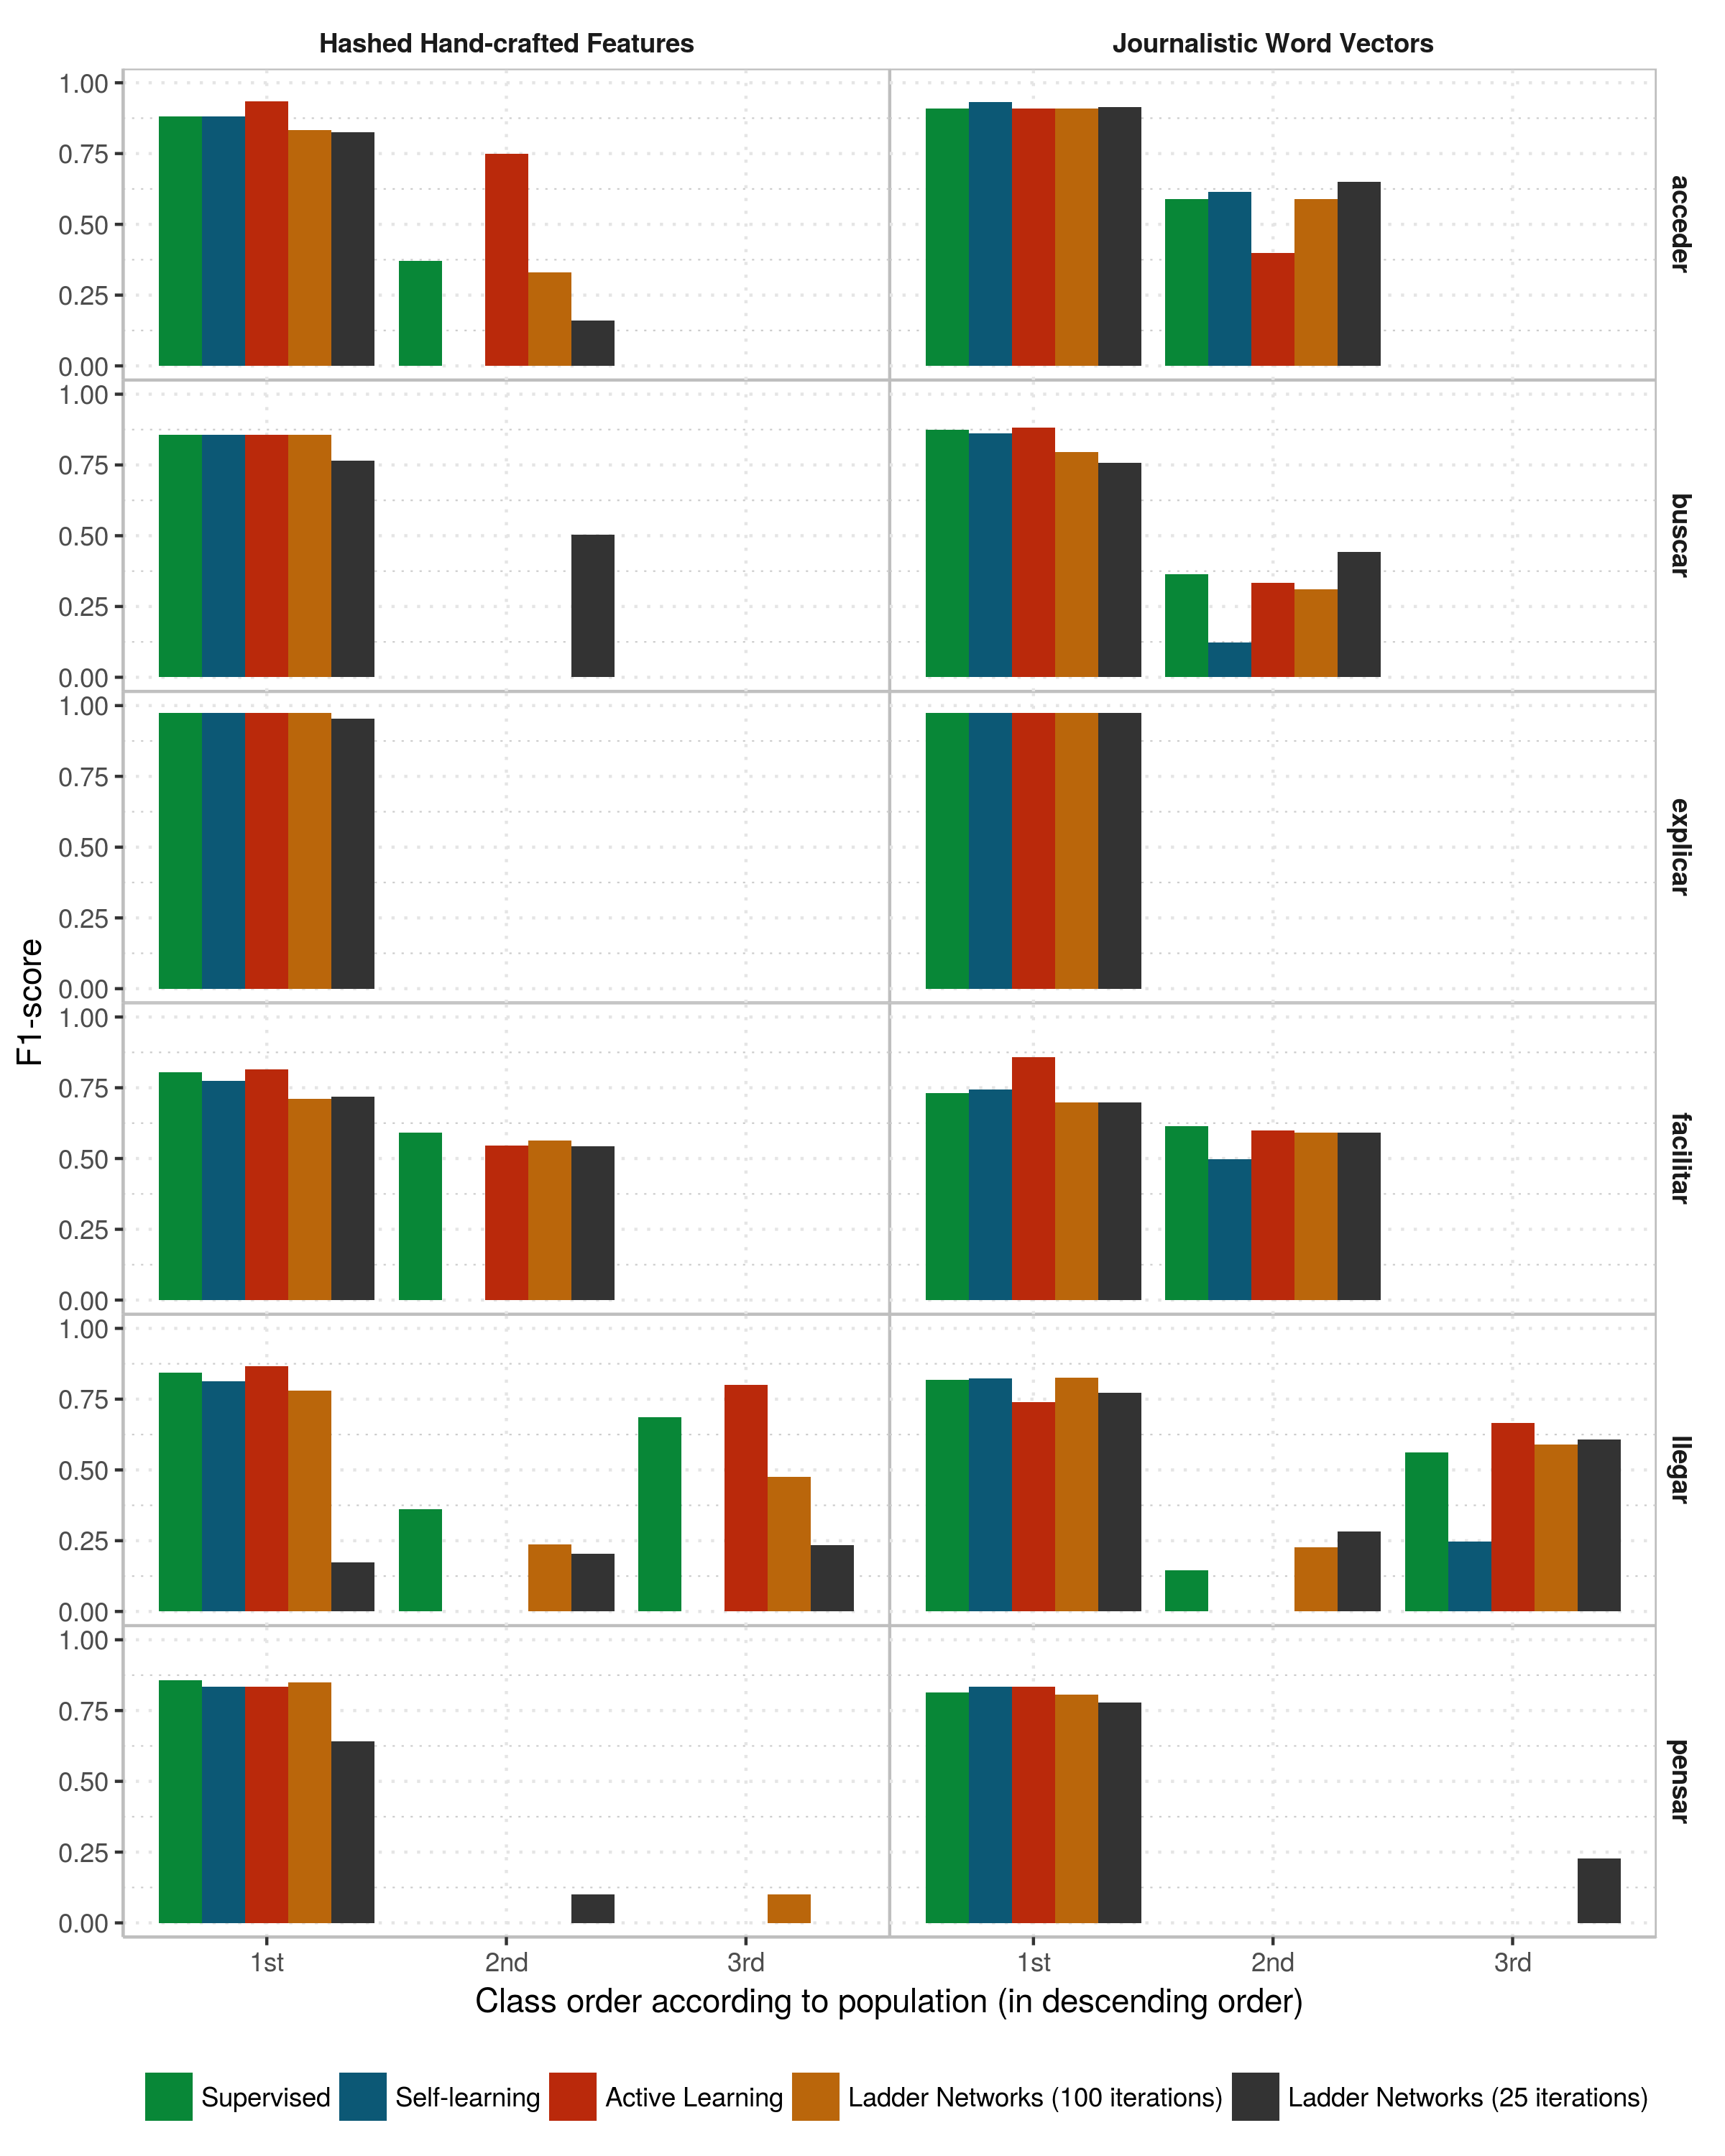
\includegraphics[height=0.9\textheight,width=\textwidth,keepaspectratio]
    {plots/ladder/per_sense_fscore}
  \caption{Comparison of macro and weighted average F1-score for supervised,
  self-learning, active learning, and ladder networks (using 100 iterations
  first and using 25 iterations secondly)}
  \label{fig:ladder:performance}
\end{figure}

Figure \ref{fig:ladder:performance} shows the F1-score macro and weighted
average for supervised, self-learning, active learning, and ladder networks
(using 100 iterations) over the test dataset. In this case, ``supervised'' is
the evaluation of the model in the initial iteration of any of the wrapper
algorithms (as it is the same for both, i.e. only using the manually labeled
data). The self-learning/active learning/ladder networks bars represent the
performance of the model over the held-out test dataset after finishing the
iterations of the corresponding algorithm. The structure of the graphic is as
follows:

\begin{itemize}
  \item Each row shows the results for a token lemma: ``acceder'', ``buscar'',
    ``explicar'', ``facilitar'', ``llegar'', and ``pensar''.
  \item Each column stands for a feature representation: hand-crafted hashed
    features and journalistic word vectors.
  \item Each group of bars in each plot represents the class (i.e. sense) for
    that lemma. These are ordered according to number of occurrences of the
    class in the dataset.
  \item Each bar plot in a different color inside a group represents the
    algorithm: supervised (i.e. evaluation moment of the initial iteration for
    a wrapper algorithm, in this case self-learning), self-learning (i.e.
    evaluation moment of the final iteration after self-learning finishes),
    active learning (i.e. evaluation moment of the final iteration after active
    learning finishes), and two versions of ladder networks (i.e.
    distinguishing different moments when the ladder networks algorithm stops,
    in this case after reaching 100 or 25 iterations).
  \item The height of the bar represents the value of the F1-score per each
    class.
\end{itemize}

Once again, recall that only the last two rows of the graphic represent the
lemmas with 3 senses (i.e. ``llegar'' and ``pensar''). The first four lemmas
can at most show results for two senses.

Note that ladder networks (in either case) performs equally or even better than
active learning in most of the senses. Remember that so far active learning
have shown the best results as it can be appreciatted in the Figure.

Moreover, there are a couple of cases where the ladder network (with 100 or 25
iterations) performs better than supervised learning on a class that supervised
learning does not recognize at all (e.g. the third most frequent class of the
lemma ``pensar''). Of course this might happen by random chance, but it is
still something to consider as ladder networks, unlike active learning, is
completely automatic (i.e. there is no human involvement). Moreover it happens
differently for ladder networks using 100 iterations and using 25 iterations.

Clearly, ladder networks is also a better alternative (or at least has better
performance) than self-learning. And it also has better performance using word
embeddings than using hand-crafted features, as we have seen along this thesis.

Notice also that in general (specially for word embeddings) stopping ladder
networks at 25 iterations has better performance than going the full 100
iterations. As I will show further, around 25 iterations begins the drift to
the most frequent class which is a good indication that this is why ladder
networks with only 25 iterations performs better than with 100 iterations.
Notice specially that ladder networks with 25 iterations tend to perform worse
than ladder networks with 100 iterations for the case of the most frequent
class. This is yet more evidence that stopping the algorithm when it begins to
drift to the most frequent class is a good solution to the problem of having
worse performance for less frequent classes.

In summary, ladder networks present some impressive results, specially in
comparison to active learning and taking into account that it is a purely
automatic method. It has much better results also than self-learning and it
seems that more insightful diagnostics over the iterations of the algorithm can
help balance the performance for the classifier on classes besides the most
frequent one. 

Even if ladder networks are not the best solution for all the cases, it is
clear that being a semi-supervised method that is completely automatic, it
improves on what other methods can achieve. E.g. the model has more
information, and thus more coverage, than a purely supervised method, and it
also avoids the use of an oracle for the annotation procedure. From these
results I accept Hypothesis \ref{hyp:ladder:1} that ladder networks improves
over the purely supervised or other semi-supervised methods. It can be argued
that, even if the raw performance of the purely supervised approach and the
active learning approach is comparable to that of ladder networks, the latter
are less expensive than active learning and in general do a better job of
maintaining good performance in all classes.

\subsection{Hypothesis \ref{hyp:ladder:2}}\label{sec:ladder:hyp:2}

Hypothesis \ref{hyp:ladder:2} was planned to compare how ladder networks work
when facing a similar task to that of the wrapper algorithms I explored in the
previous chapters. The hypothesis states that the representativity of the
classes if using the model to classify some unsupervised data will be
maintained through the iterations. In particular, it was in the visualization
of this experiment's results that I found that around iteration number 25 there
was a drifting of the algorithm to the most frequent class. In this section
there are two plots of the same results, varying only in the number of
iterations the ladder network algorithm is given to finish.

Like for self-learning and active learning in the previous chapter, to analyze
these results I use two forms of visualization: one explores the distribution
of the classes along the iterations of the algorithm and the other explores the
proportional count of each class added on each iteration of the algorithm.

\subsubsection{Classes' population distribution across iterations}

\begin{figure}[htb!]
  \centering
  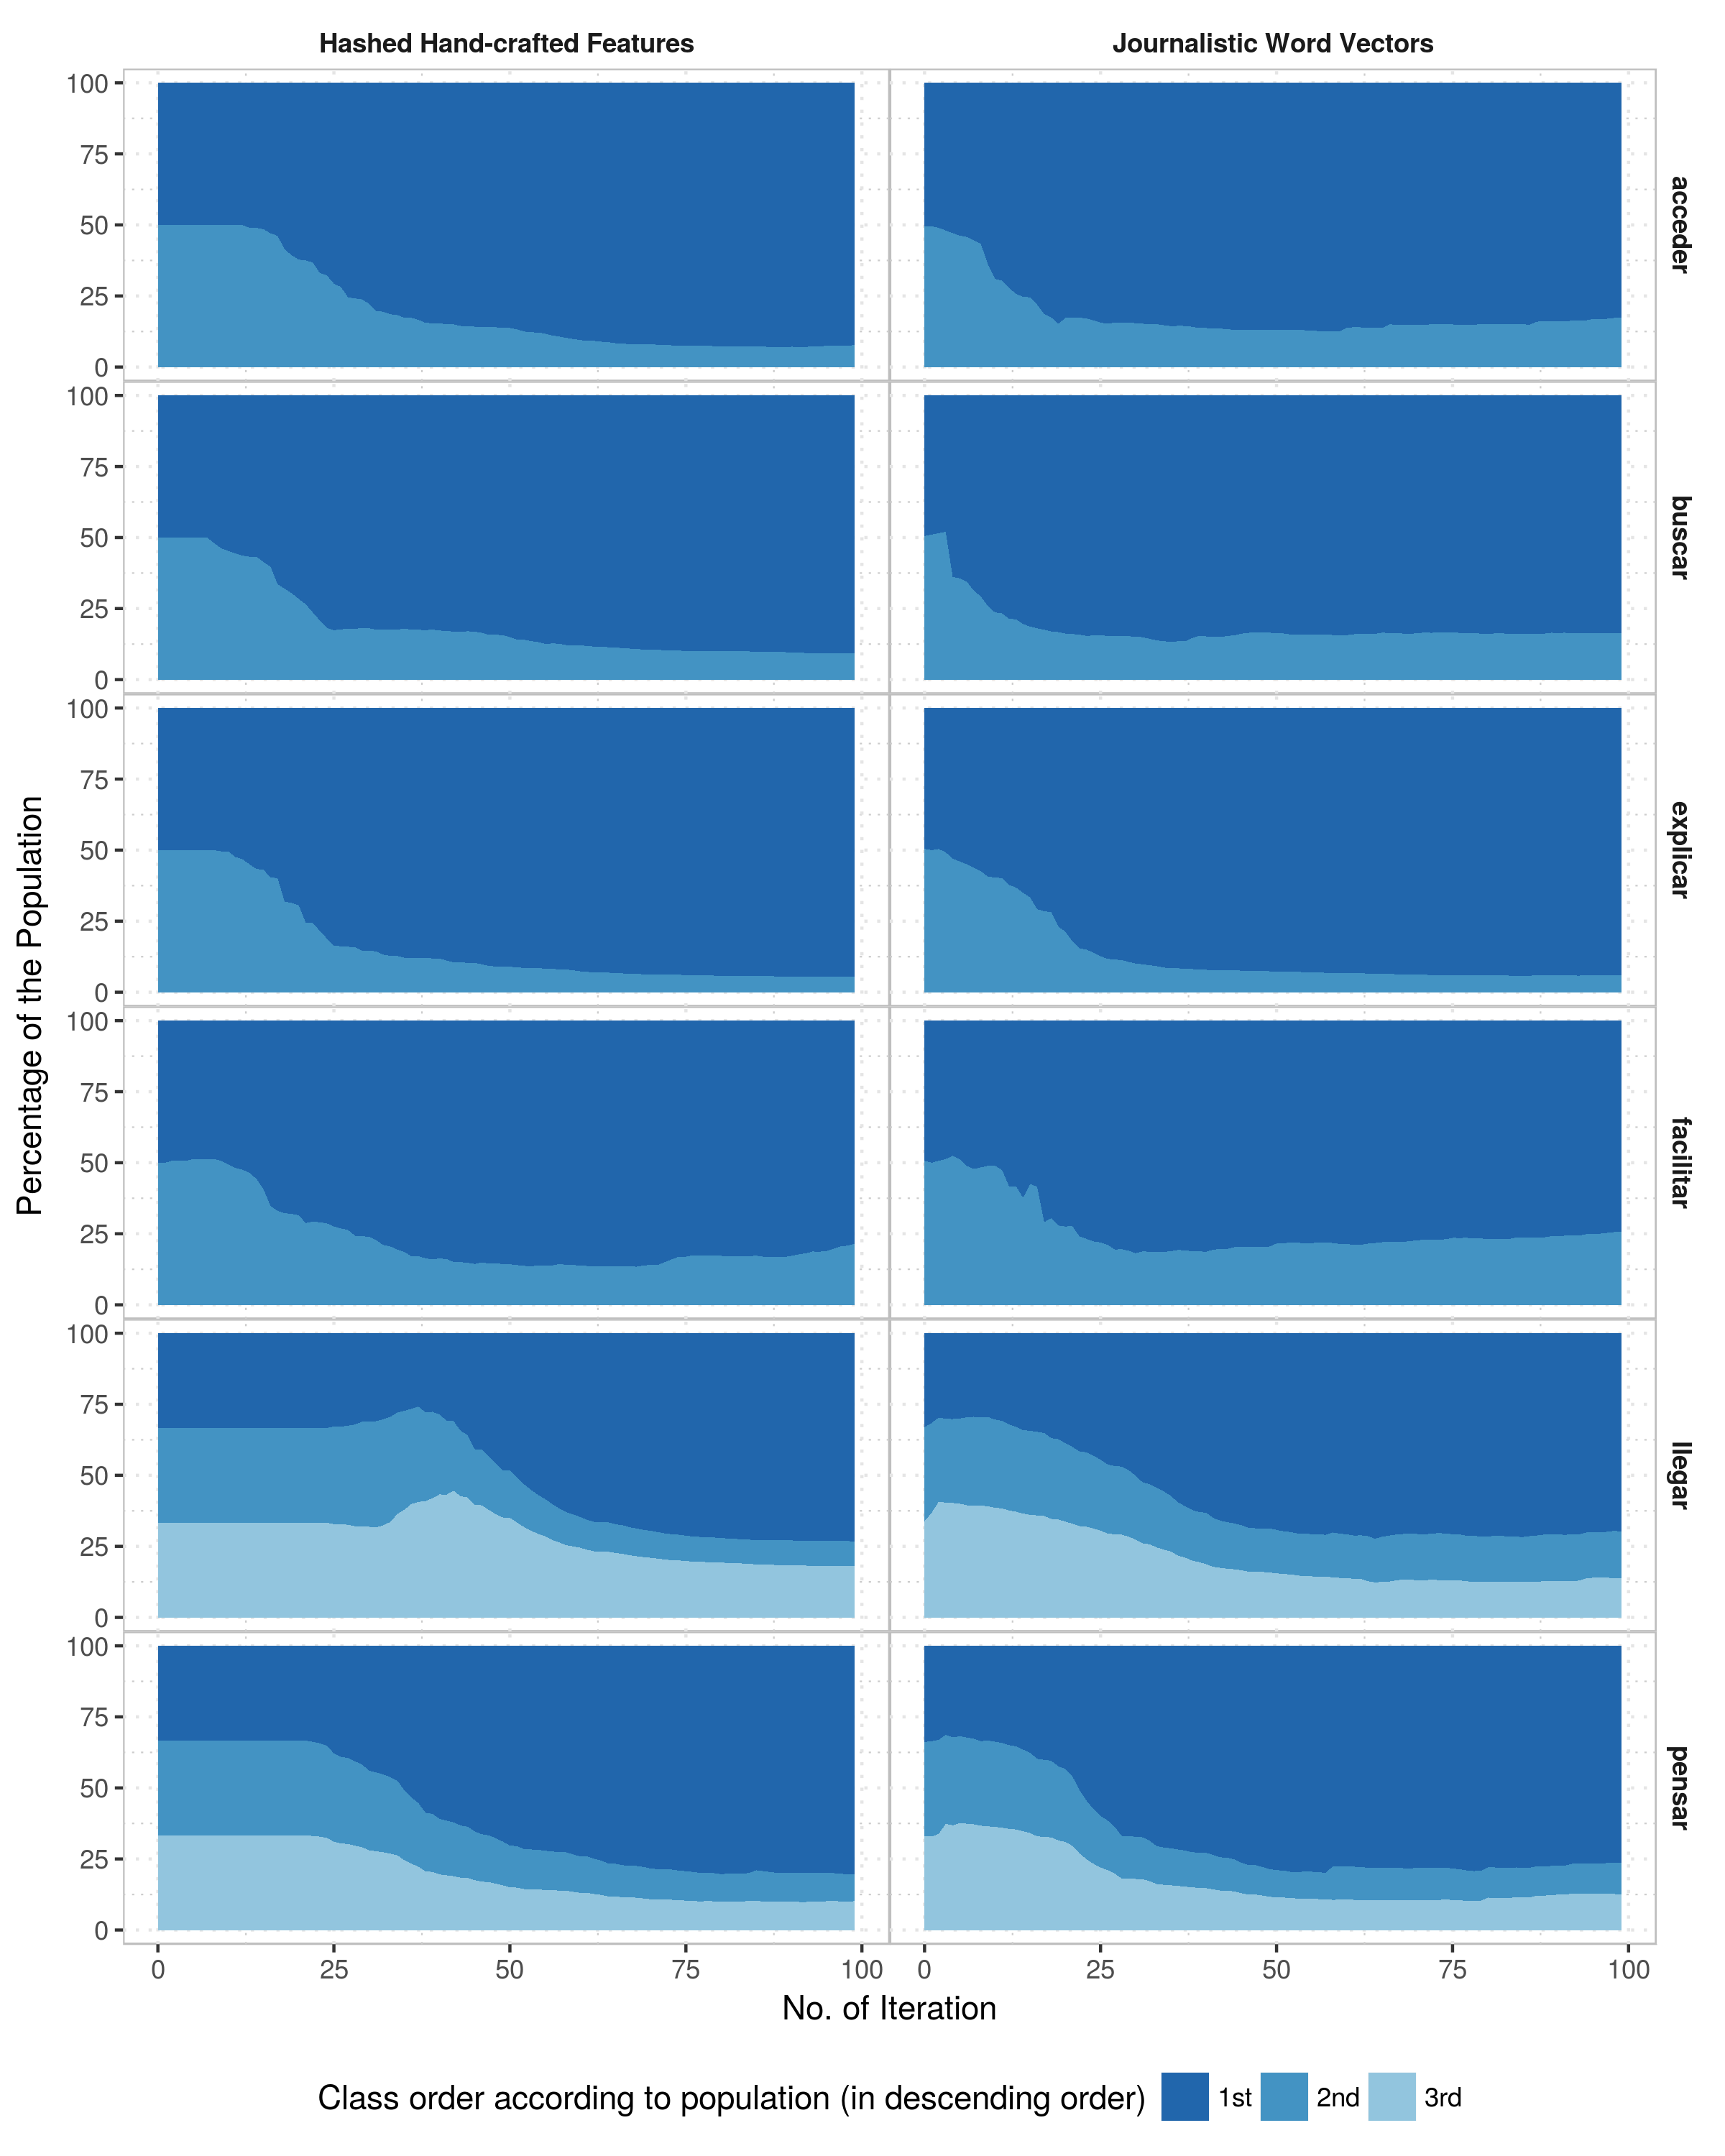
\includegraphics[height=0.9\textheight,width=\textwidth,keepaspectratio]
    {plots/ladder/population_distribution_100}
  \caption{Distribution of the classes' population across ladder networks
  algorithm's iterations (with a maximum of 100 iterations) as a proportion of
  the whole training dataset}
  \label{fig:ladder:population_distribution:100}
\end{figure}

\begin{figure}[hb!]
  \centering
  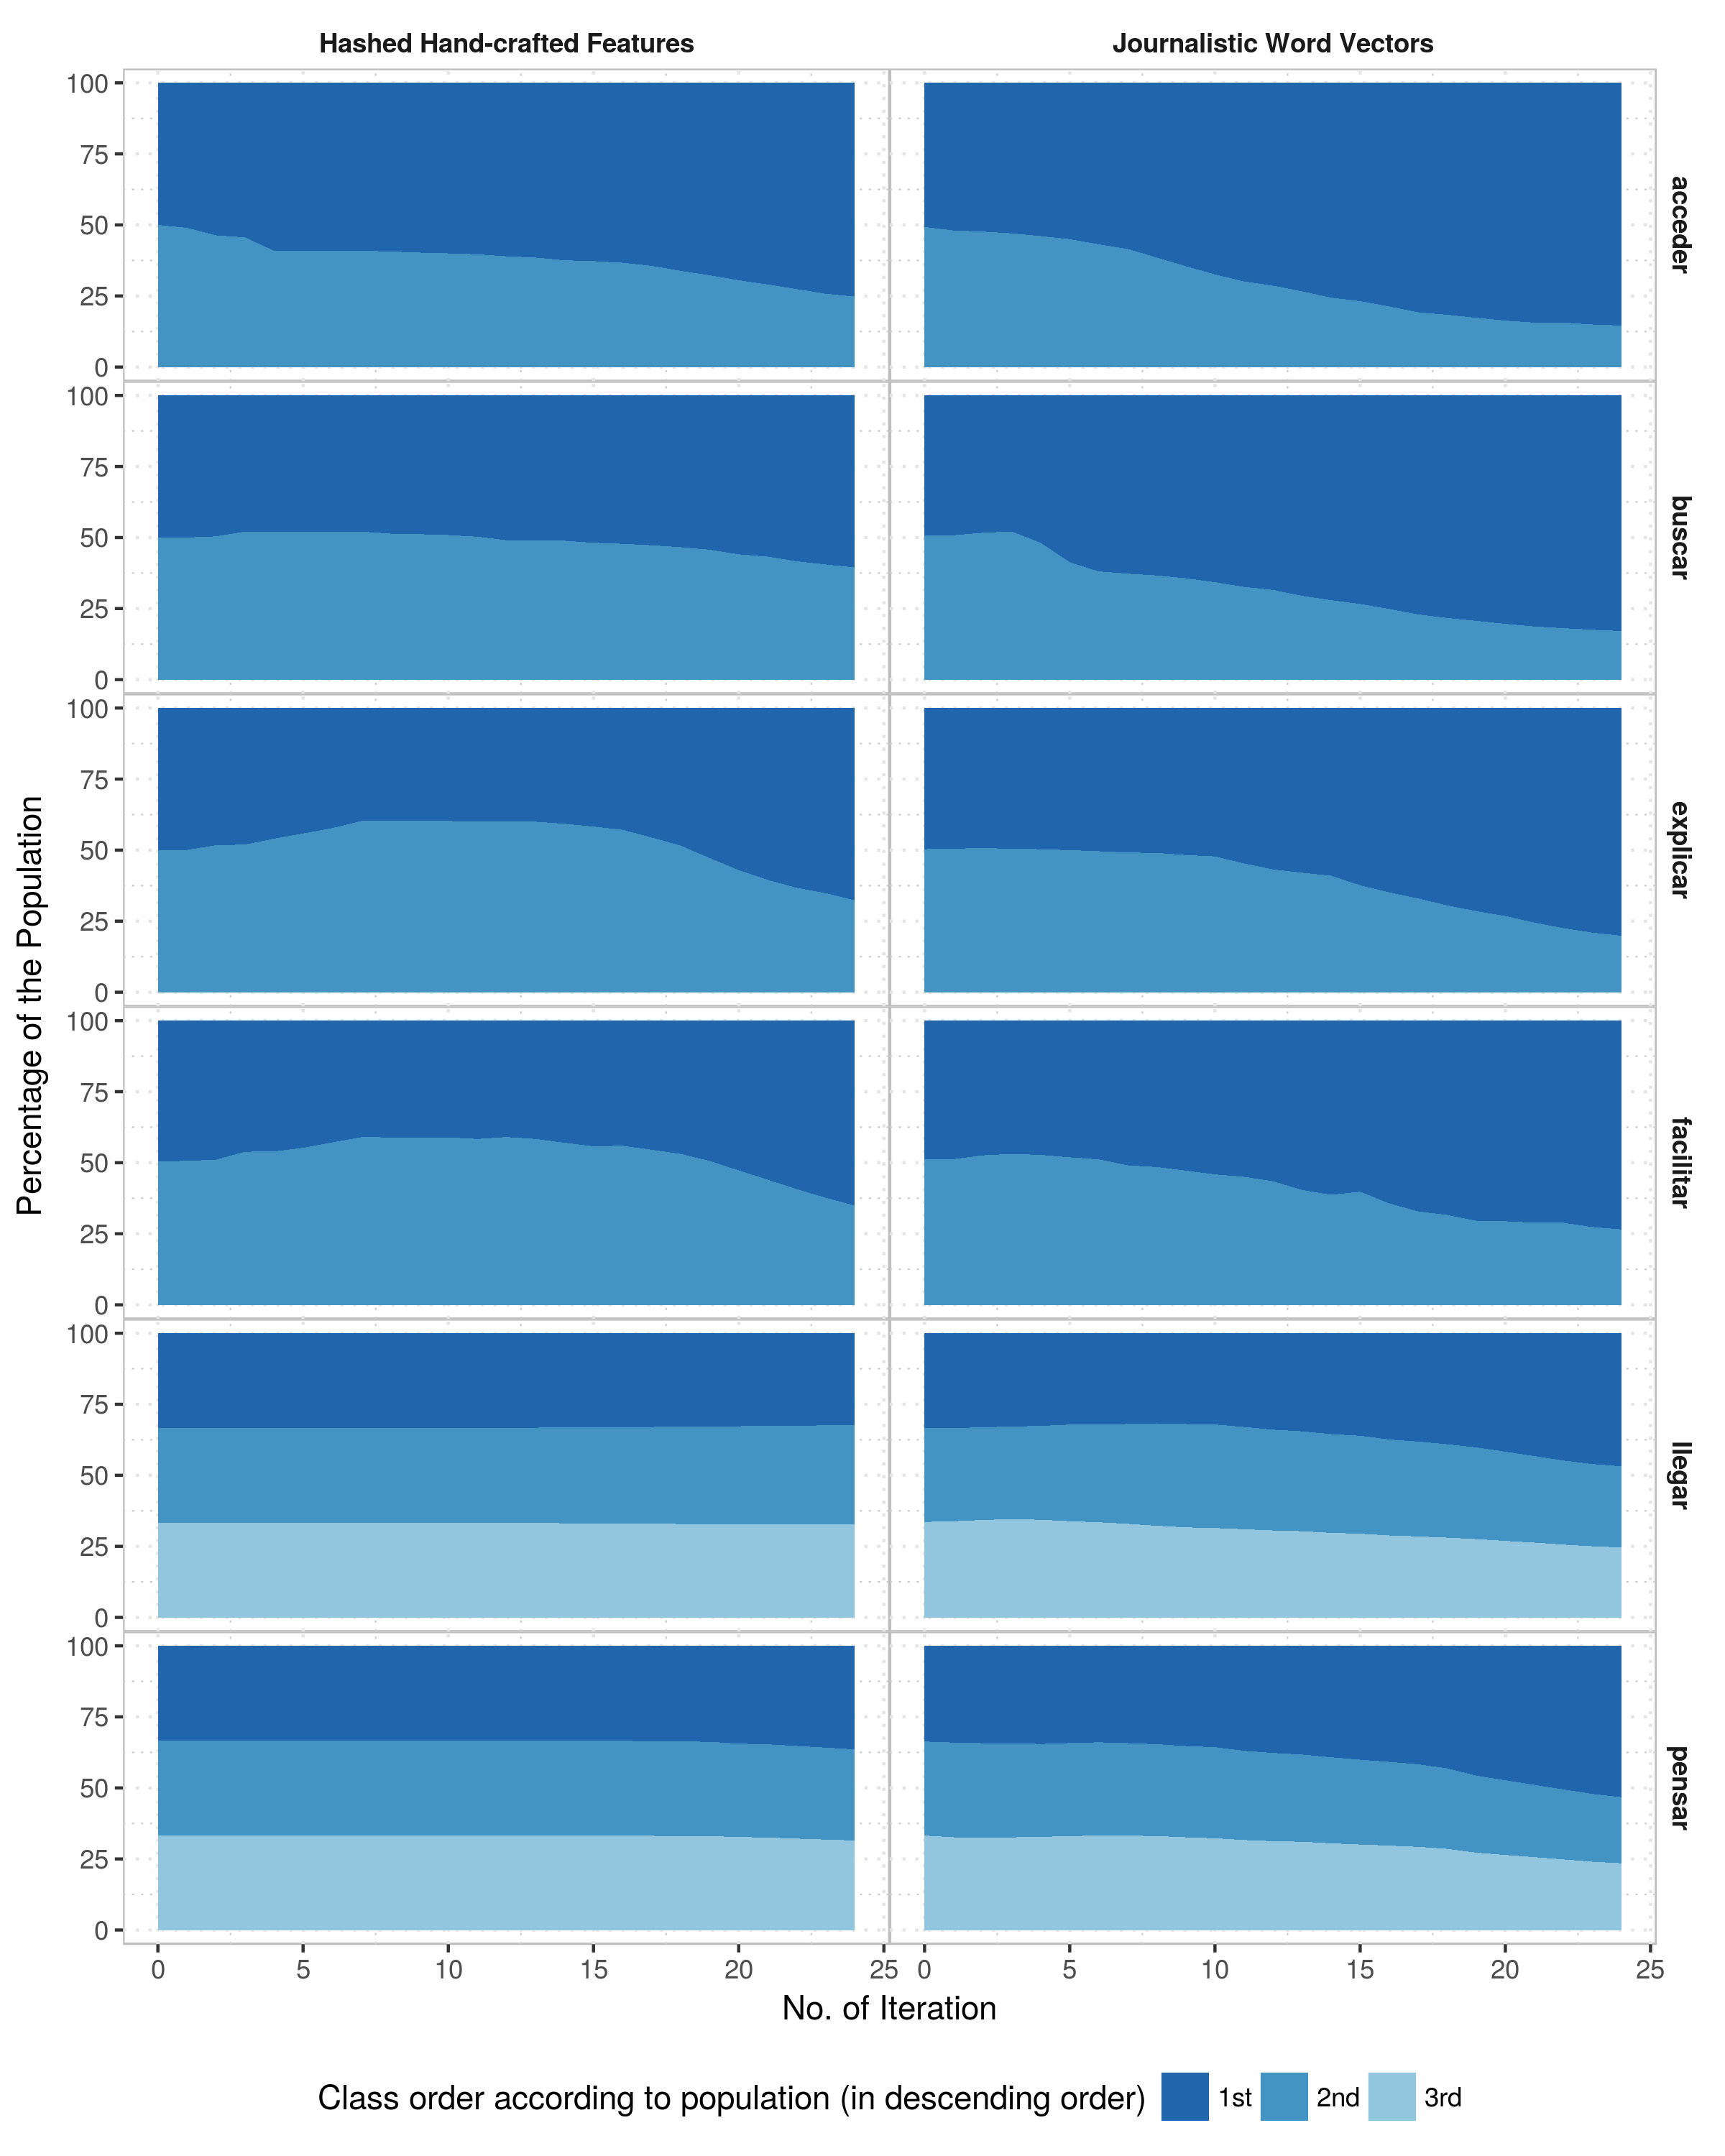
\includegraphics[height=0.9\textheight,width=\textwidth,keepaspectratio]
    {plots/ladder/population_distribution_25}
  \caption{Distribution of the classes' population across ladder networks
  algorithm's iterations (with a maximum of 25 iterations) as a proportion of
  the whole training dataset}
  \label{fig:ladder:population_distribution:25}
\end{figure}

Figure \ref{fig:ladder:population_distribution:100} shows the distribution of
the population of the classes across ladder network iterations (with a maximum
of 100 iterations) of the algorithm. Each class's population is represented as
the proportion of the total number of examples in the training dataset for that
iteration. The plot is a stacked area plot that follows this structure:

\begin{itemize}
  \item Each row shows the results for a token lemma: ``acceder'', ``buscar'',
    ``explicar'', ``facilitar'', ``llegar'', and ``pensar''.
  \item Each column stands for a feature representation: hand-crafted hashed
    features and journalistic word vectors.
  \item The x-coordinate represents the iteration in the self-learning
    algorithm.
  \item The y-coordinate represents the percentage of population.
  \item Each area of a different color represents the proportion of examples
    for each of the classes in the dataset. The classes again are ordered
    according to number of examples in the original supervised dataset.
\end{itemize}

As I already explained in previous sections of this chapter, it is around the
iterations number 25 (although not in all cases, in some cases is much earlier
and in some is later) that the distribution of the classes from the labeled and
automatic annotated classes of the unlabeled corpus used for the task (as
described in Experiment \ref{exp:ladder:3}) begin to drift to the most frequent
class. Once again, the prevalence of the most frequent class is more acute for
hand-crafted features than for journalistic word embeddings.

If I decide to stop the algorithm by the iteration number 25, the distribution
of classes looks like the one in Figure
\ref{fig:ladder:population_distribution:25}. The figure has the exact same
structure as the previous figure with the only difference being in the maximum
number of training iterations of the ladder network model.

In this case however, the drift of the model to automatically annotate
everything as the most frequent class is not so strong as in the previous
figure. The algorithm stops before that happens (although there are exceptions,
after all, like all, each lemma has its own set of properties the algorithm
needs to adapt to).

In any case, the drifting of the ladder network model to the most frequent
class is not as strong as in self-learning, where it is practically immediate,
right after the first iteration. This can well be a consequence of the ladder
network learning the model through the iterations as it slowly gains confidence
of the decision boundaries. Unlike in self learning, the use of unlabeled data
in this case serves to delay and avoid the drift to the most frequent class.

Eventually, with more iterations, the most frequent class starts gaining more
and more probability, which is expected as the data has a Zipfian distribution.
However, the fact that the results on the test dataset are better than those
for self-learning seems to indicate that the ladder network is actually
classifying the examples of the most frequent class correctly (better
precision), unlike self-learning, which might well classify them as majority
class just because it cannot tell them apart from any other class.

\subsubsection{Population added per sense per iteration}

\begin{figure}[hb!]
  \centering
  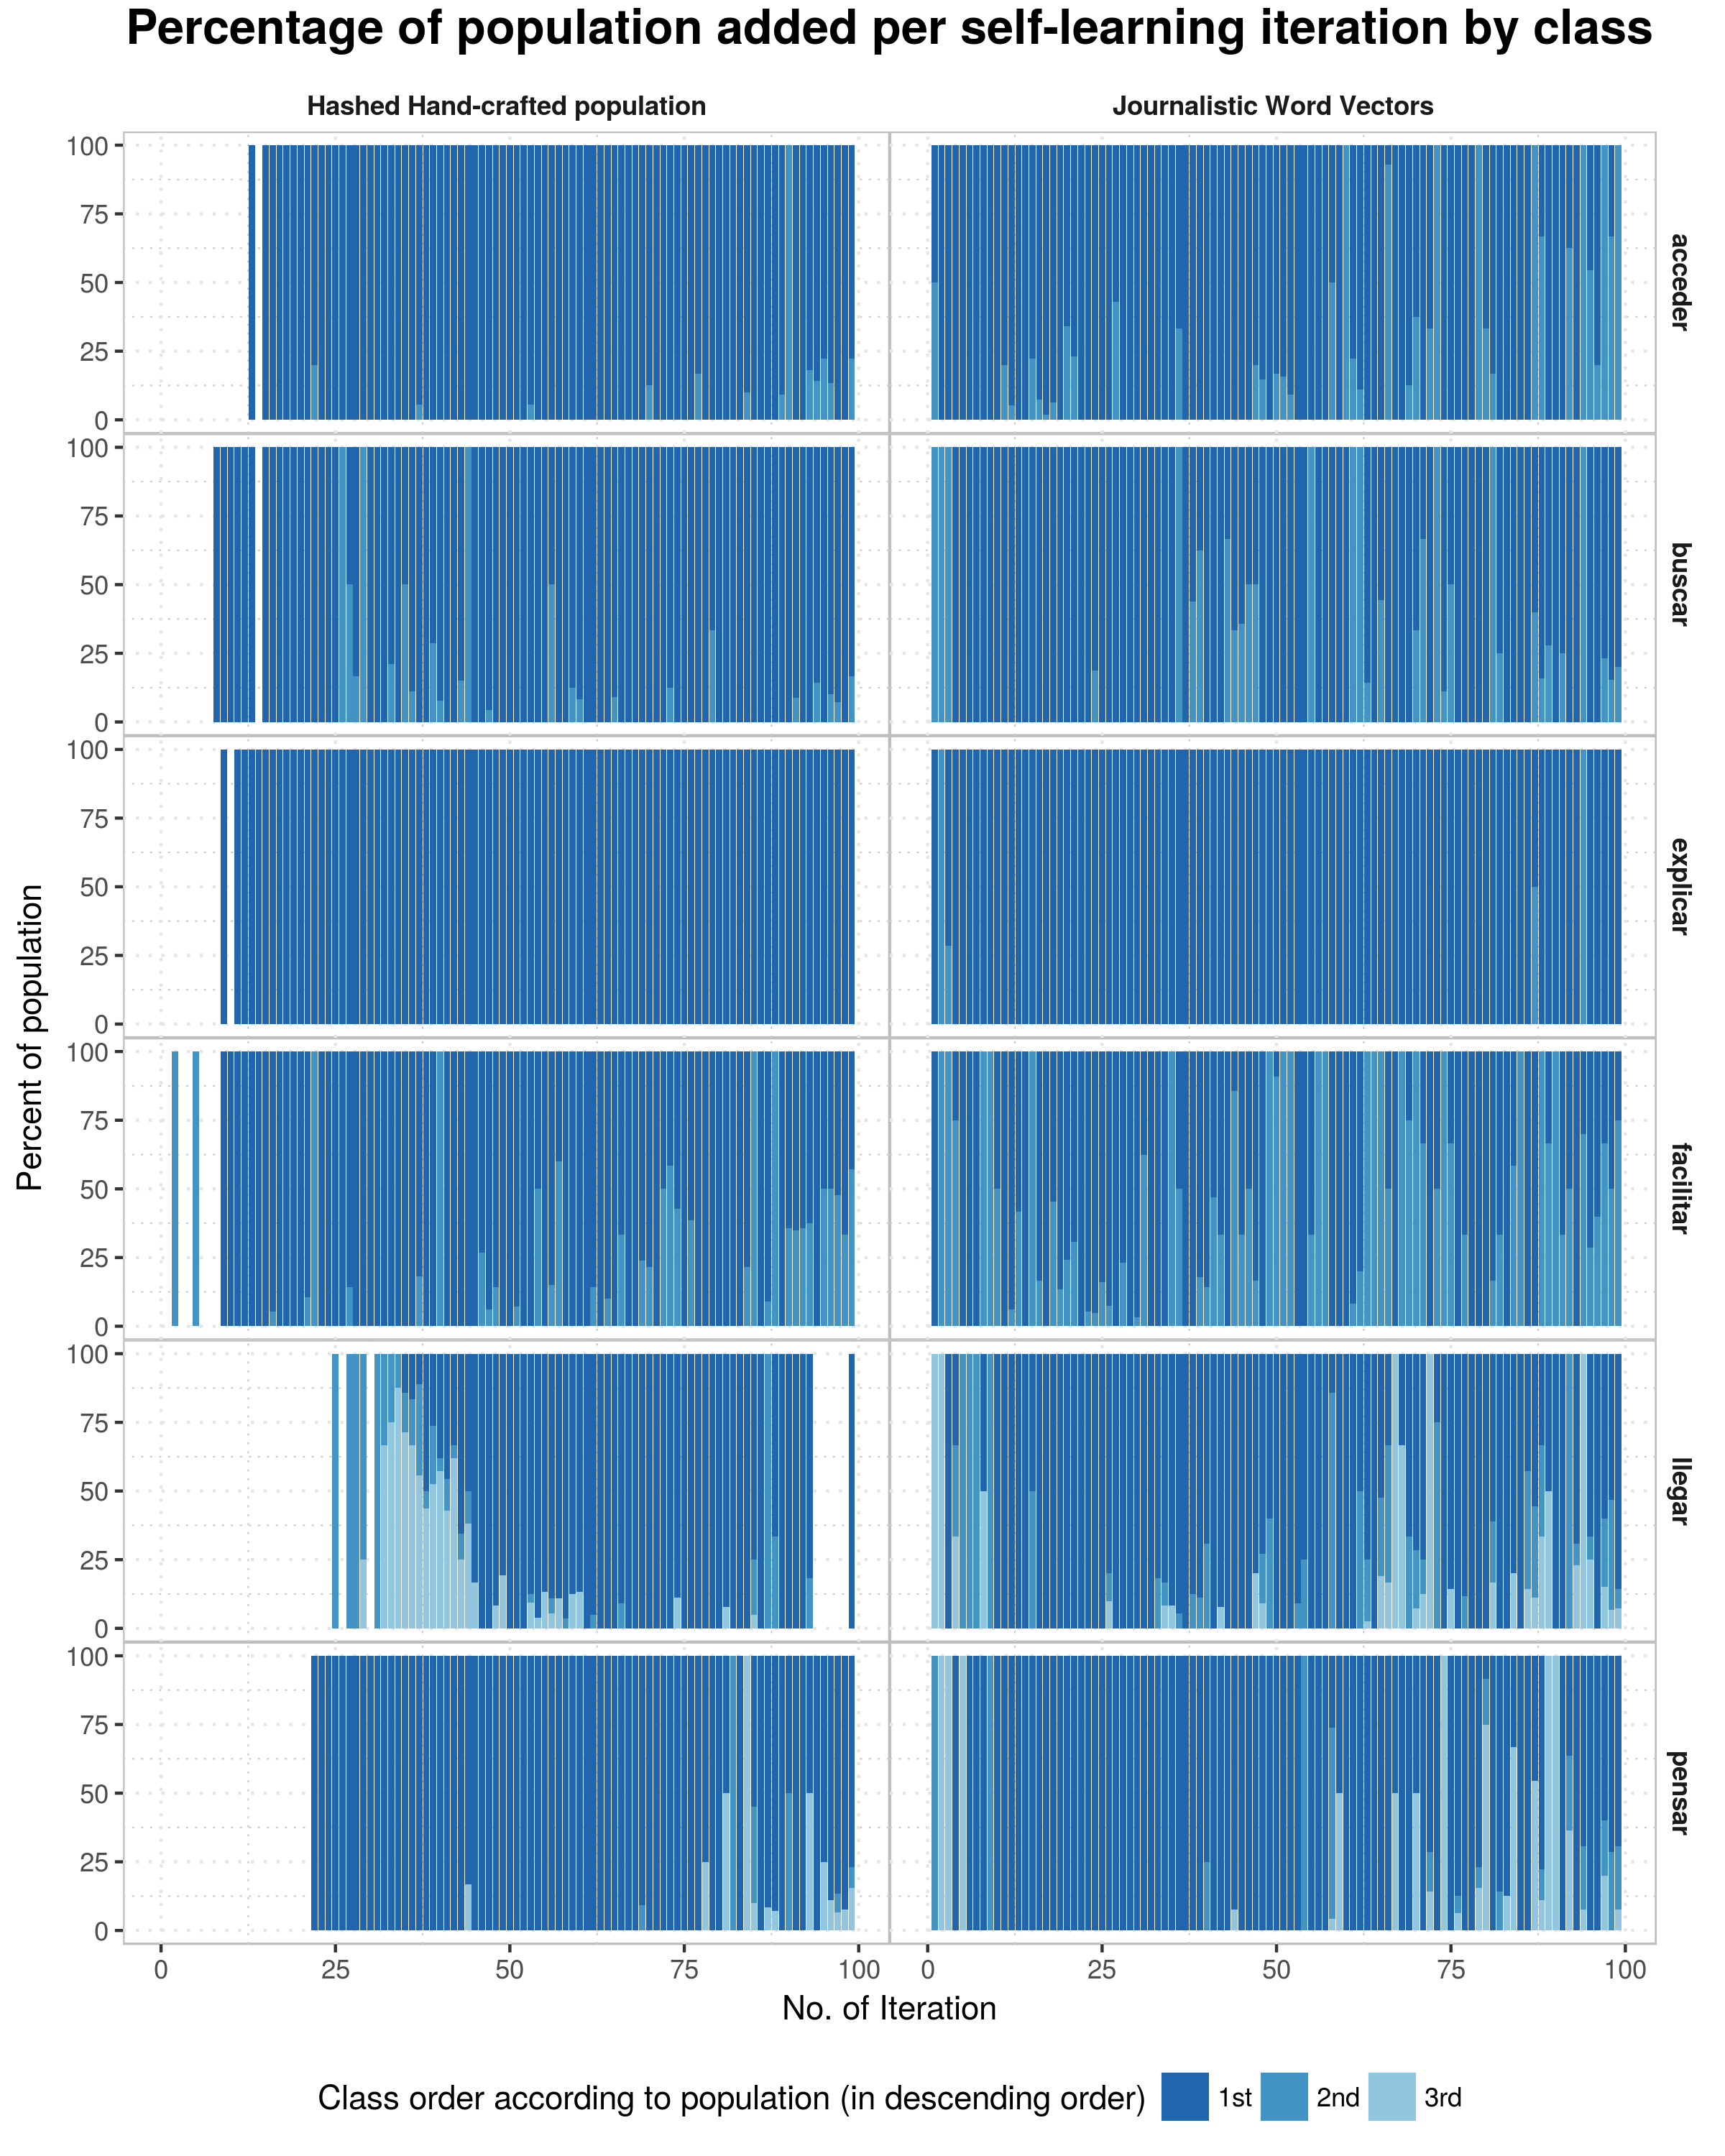
\includegraphics[height=0.9\textheight,width=\textwidth,keepaspectratio]
    {plots/ladder/population_add_per_class_100}
  \caption{Population added per sense on each iteration of ladder network (with
  a maximum of 100 iterations) as a proportional count of all the examples
  added in that iteration}
  \label{fig:ladder:population_add_per_class:100}
\end{figure}

\begin{figure}[htb!]
  \centering
  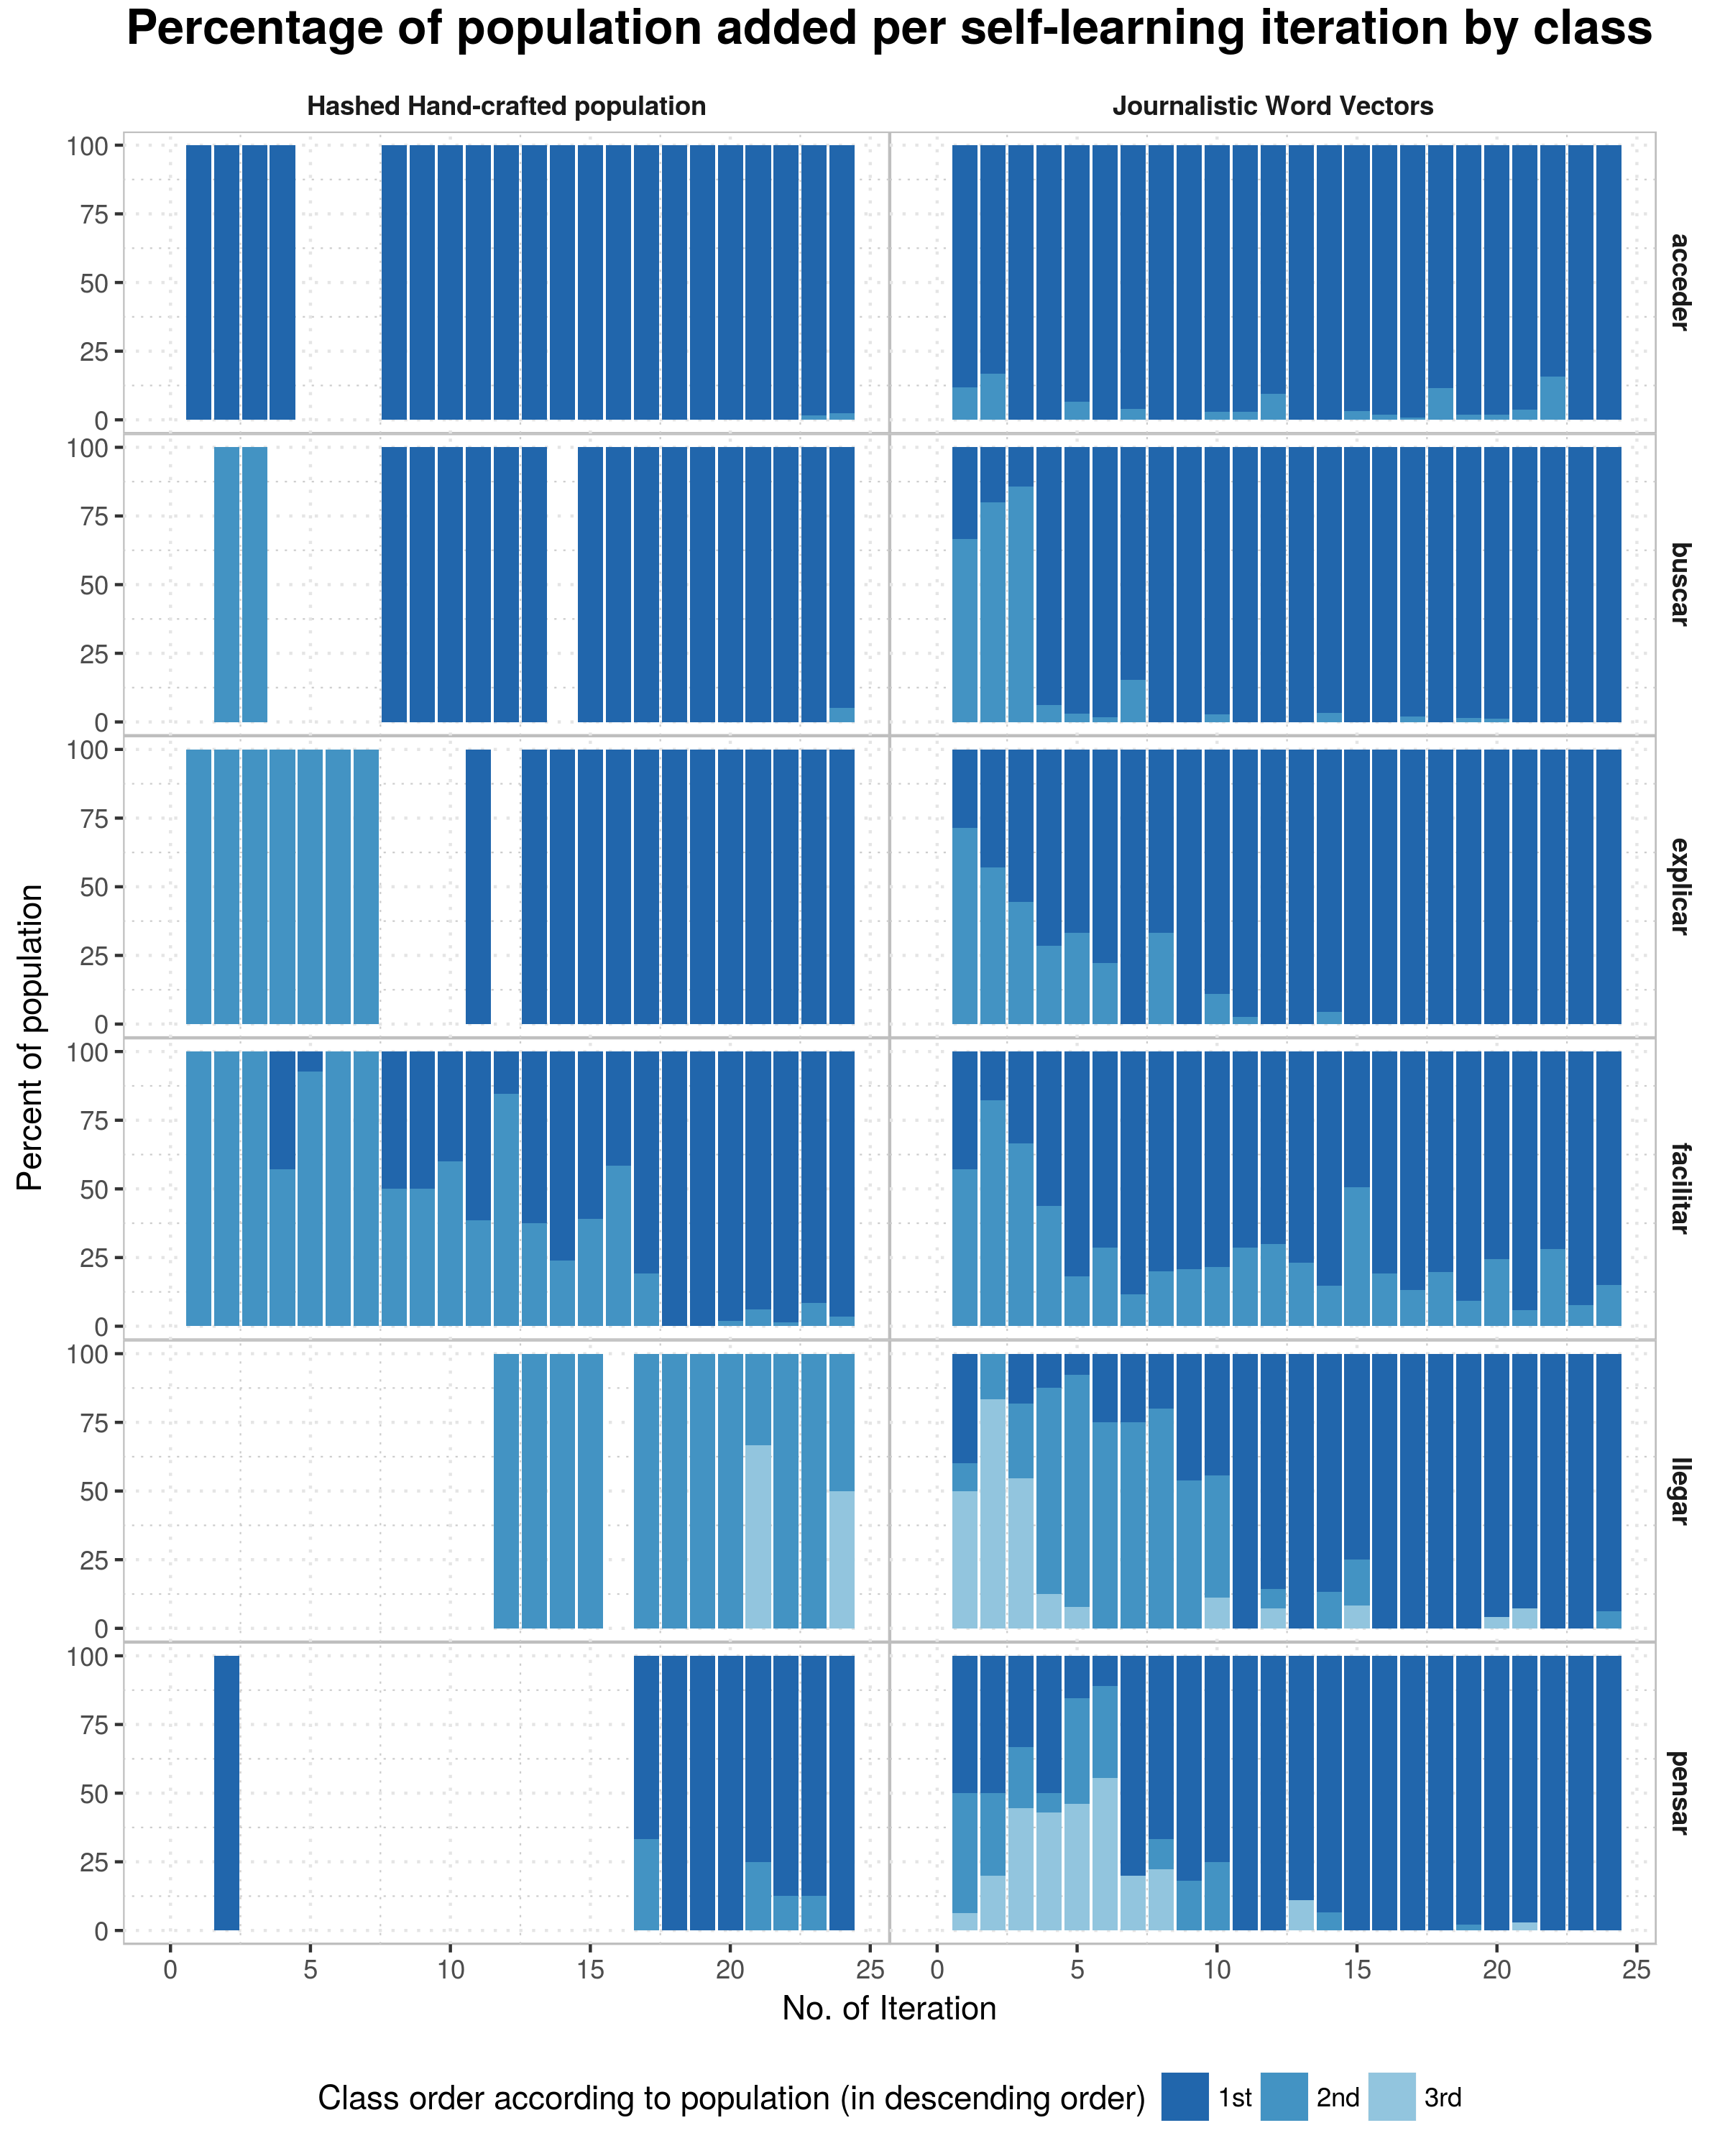
\includegraphics[height=0.9\textheight,width=\textwidth,keepaspectratio]
    {plots/ladder/population_add_per_class_25}
  \caption{Population added per sense on each iteration of ladder network (with
  a maximum of 25 iterations) as a proportional count of all the examples
  added in that iteration}
  \label{fig:ladder:population_add_per_class:25}
\end{figure}

Figure \ref{fig:ladder:population_add_per_class:100} shows the proportion of
examples added per class on each iteration. It is a stacked bar plot where each
bar represents the total examples added in the iteration split by the
proportion of classes automatically annotated as such. The structure of the
plot is the following:

\begin{itemize}
  \item Each row shows the results for a token lemma: ``acceder'', ``buscar'',
    ``explicar'', ``facilitar'', ``llegar'', and ``pensar''.
  \item Each column stands for a feature representation: hand-crafted hashed
    features and journalistic word vectors.
  \item The x-coordinate represents the iteration in the self-learning
    algorithm.
  \item The y-coordinate represents the percentage of examples automatically
    annotated for each sense.
  \item Each bar plot represents the distribution of the examples annotated in
    the iteration. Each color of the stacked bar represents the class with
    which the examples were annotated.
\end{itemize}

Similarly, Figure \ref{fig:ladder:population_add_per_class:25} shows the same
information but this time for the ladder network algorithm stopping at 25
iterations.

The first thing to note from these Figures is that, in this case, unlike in the
same figures of previous chapters, there are missing bars in some cases. This
is because, unlike self-learning, for the ladder network algorithm it is not
mandatory to annotate examples from the unlabeled dataset. Thus, in the first
iterations, where the algorithm generally does not annotate anything, it is
because the model is not certain enough about the annotated instances.

This is a consequence of the model not only learning from the labeled corpus,
but from the unlabeled corpus as well. The model has less certainty as the
unlabeled data, which is added in batches, adds information that avoids the
model to converge, but also to overfit the supervised dataset.

There are some lemmas on which the model has better certainty than others. In
particular the lemma ``llegar'', for the hand-crafted features representation,
is the one on which the model takes the most to begin adding examples. This
means that the model cannot handle the information from the lemma given by the
unsupervised data in the first iterations and thus takes more time to adjust
the parameters to that lemma. A quick look to Figure
\ref{fig:ladder:performance} shows that it is precisely for ``llegar'' that, at
25 iterations, the ladder network algorithm shows the worst performance. Also,
a quick look to Figure \ref{fig:active:population_distribution} in the previous
chapter shows that ``llegar'' has the highest number different senses occurring
in the unlabeled dataset. Moreover, it was the example I used when I introduced
self-learning in Chapter \ref{chapter:self-learning} to exemplify a lemma that
has one sense as most frequent in the SenSem corpus but it is not precisely the
same one as in a general corpus (thus, it is domain biased). Remember that
unlabeled instances are taken from a general domain corpus.

The lemma ``llegar'' is a particular case, and we see that the use of
hand-crafted features undermines the performance of the model over a lemma that
is so domain biased. However, it is important to note that this is not the case
for all the lemmas or even that the same happens with a less domain dependant
representation, as is the one provided by word embeddings.

Following the figures, both for 100 and for 25 iterations, it is clear that in
most of the cases the most frequent class starts to dominate the automatically
annotated examples. It is also important to notice how this is more clear for
hand-crafted features. Thus, the idea of stopping the iterations once the
ladder networks begins to drift is not so unjustified after all, specially
seeing the results given in the previous section. It is however important to
notice something: in the first couple of iterations there are more instances of
the less frequent classes, something that gradually turns over. However, it is
more notorious on the hand-crafted features that the distribution is all or
nothing, since the bars start being of one color and then suddenly turn into
the other color. This does not happen for word embeddings. In that case the
representativity of each of the classes is more uniform and more similar to the
original distribution of the classes (that is, the most frequent class is still
the most frequent, but is not the only one). Given what I have discussed over
this thesis work, it is safe to assume this is a direct consequence of the word
embeddings being able to provide a better generalization to a model.

From the results shown in this and the previous section, there is enough
evidence to accept Hypothesis \ref{hyp:ladder:2} for word embeddings. However,
there is not enough evidence to accept it for hand-crafted features.

\subsection{Hypothesis \ref{hyp:ladder:3}}\label{sec:ladder:hyp:3}

The final hypothesis of the chapter explores how the unlabeled data helps the
ladder network model reduce the tendency to overfit. Hypothesis
\ref{hyp:ladder:3} states that the overfit of the ladder network model over the
labeled data is prevented by the use of unlabeled data to calculate the global
cost function, which is composed of the labeled and unlabeled cost functions.

It is important to notice that the experiments and results shown in this
section capture the spirit of experiments on previous chapters which also
explore how adding data to a model impacts on the tendency to overfit.
However, what I could accomplish here does not directly compare to what I did
for other algorithms, such as self-learning or even the supervised methods.
This is because, unlike in those cases, the ladder networks algorithm
integrates the information from the unlabeled dataset in a different way than
the previous methods. In this case, the unsupervised information is integrated
in the weights of the network. 

\begin{figure}[htb!]
  \centering
  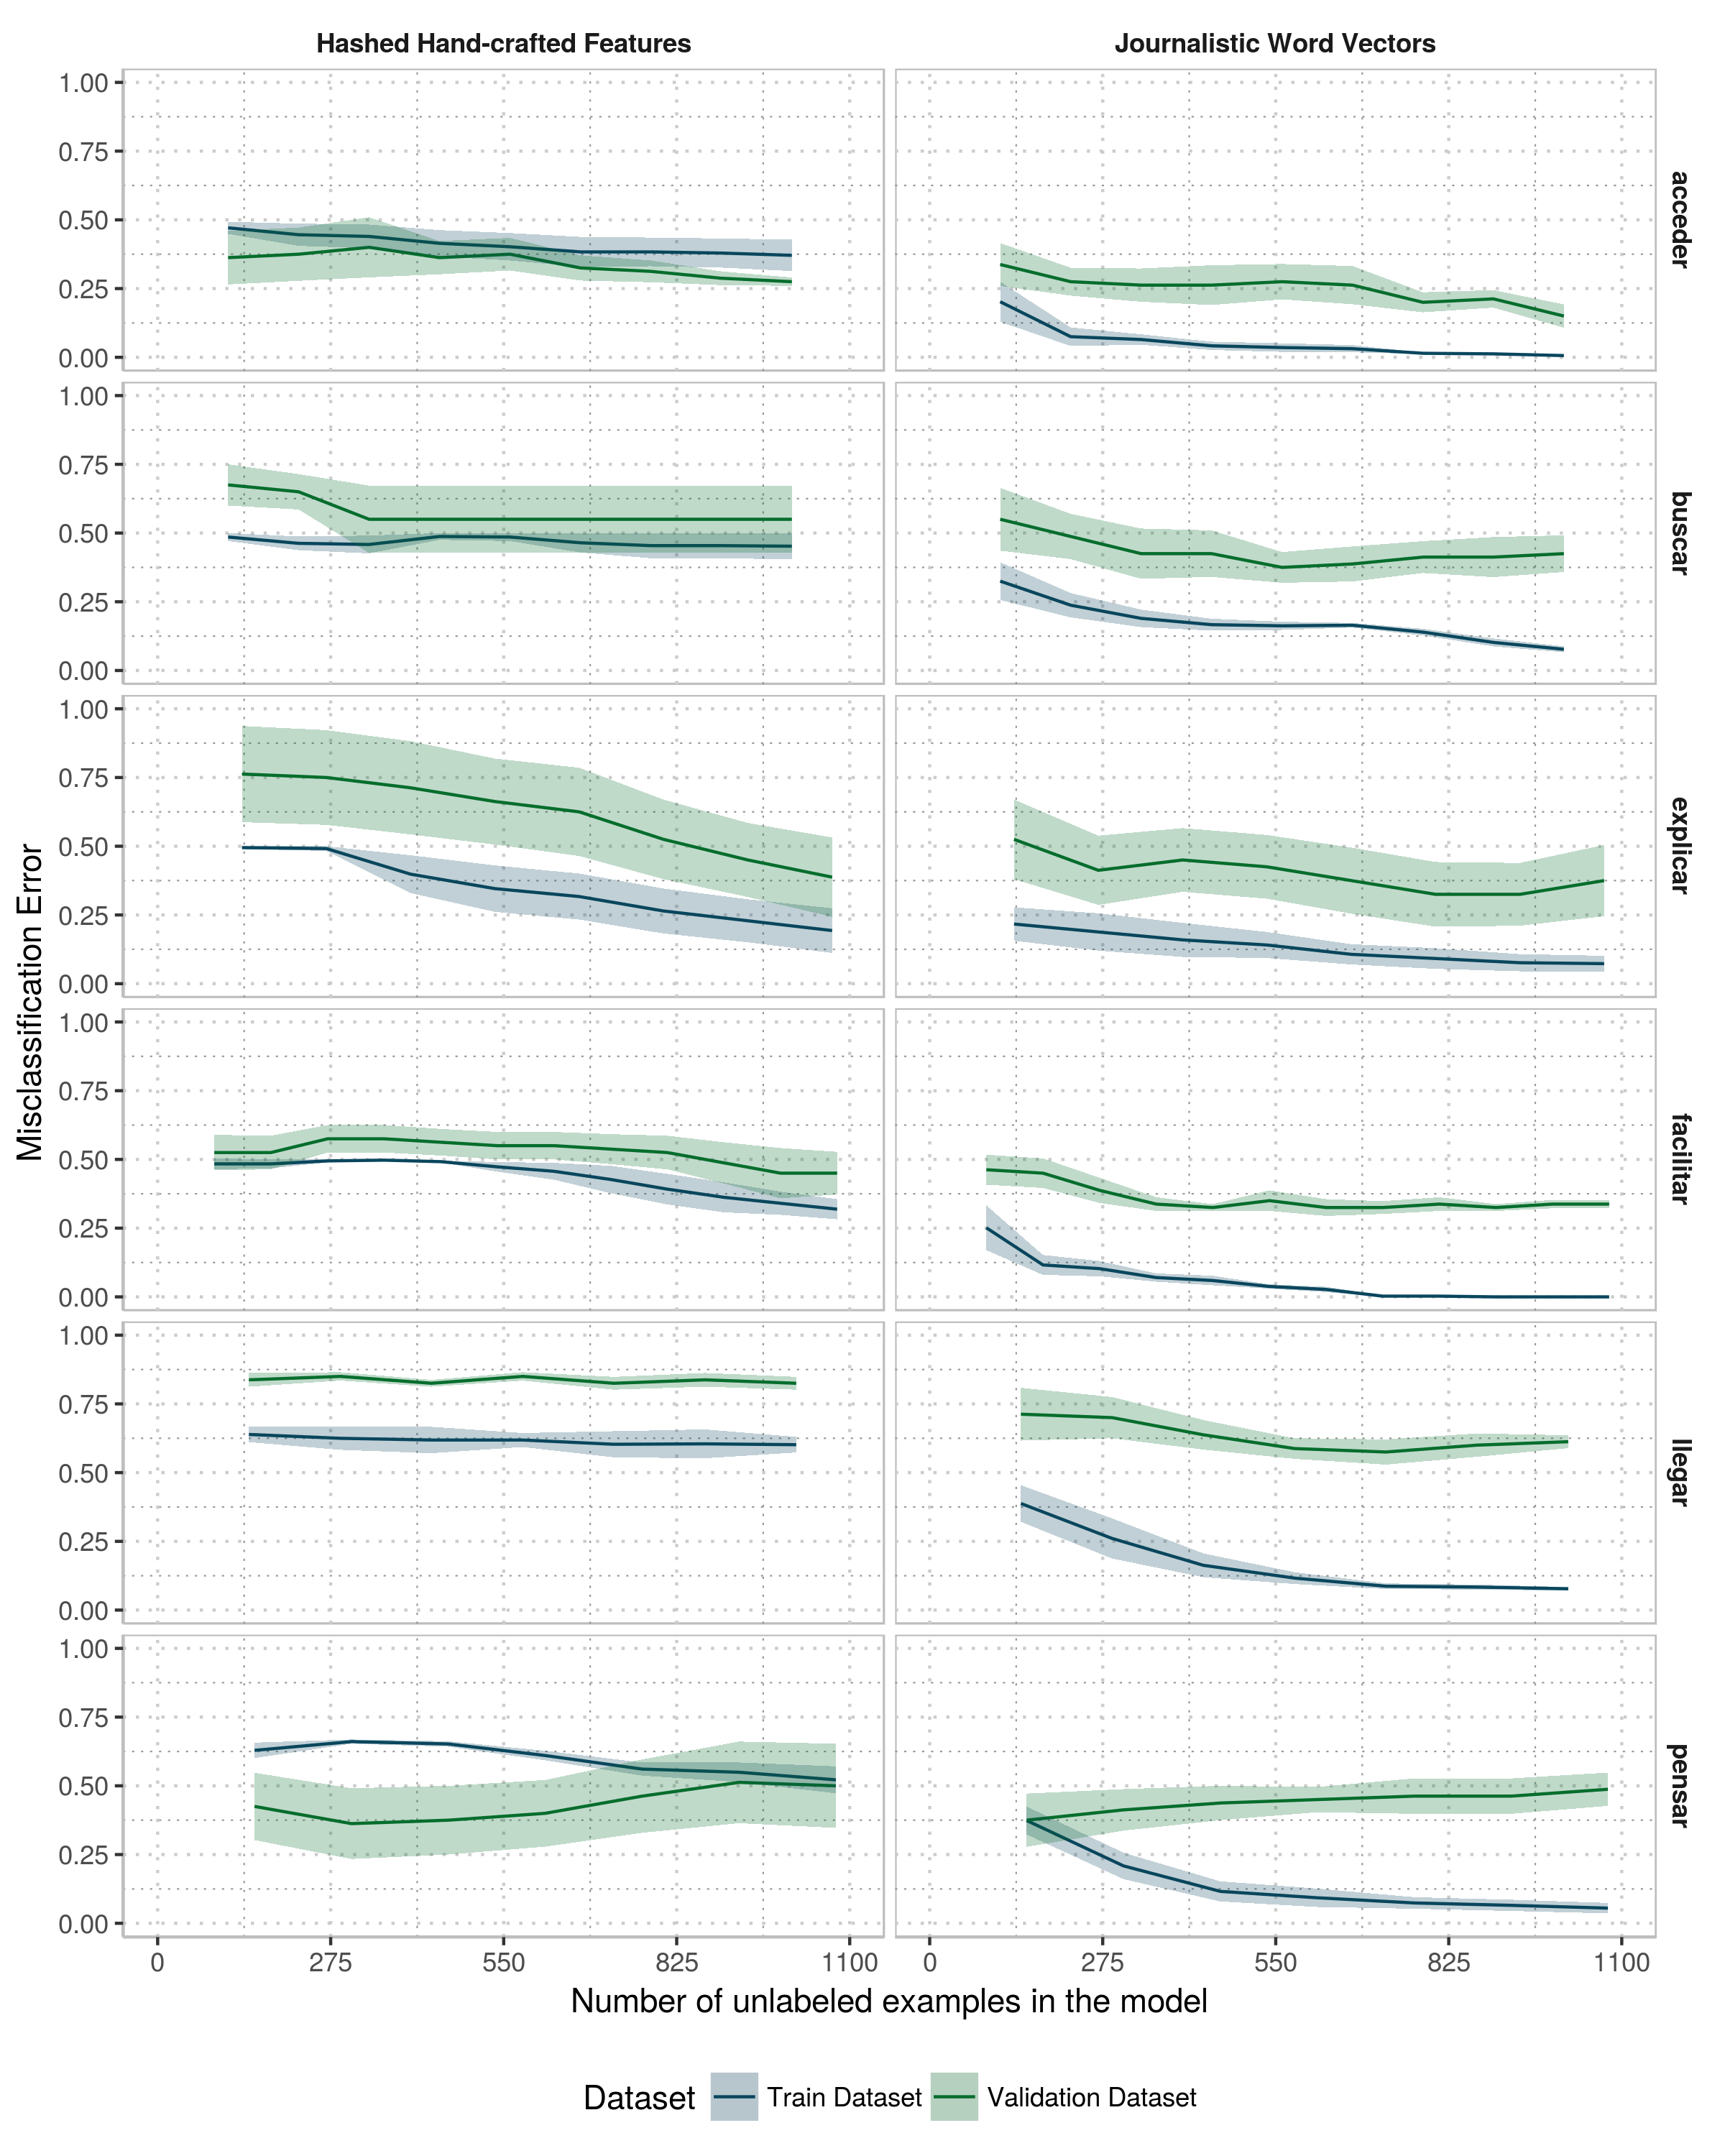
\includegraphics[height=.9\textheight,width=\textwidth,keepaspectratio]
    {plots/ladder/overfit_measure_per_examples}
  \caption{Learning curve as a function of the number of unlabeled examples
  added by the ladder network algorithm in each training iteration}
  \label{fig:ladder:overfit}
\end{figure}

Figure \ref{fig:ladder:overfit} shows the learning curve plot as a function of
the number of examples of the training dataset. The structure of the learning
curve plot is as follows:

\begin{itemize}
  \item Each row shows the results for a token lemma: ``acceder'', ``buscar'',
    ``explicar'', ``facilitar'', ``llegar'', and ``pensar''.
  \item Each column stands for a feature representation: hand-crafted hashed
    features and journalistic word vectors.
  \item The x-coordinate axis represents the number of unlabeled examples added
    in each successive iteration by the ladder networks algorithm.
  \item The y-coordinate axis represents the misclassification error.
  \item There are two colors representing the datasets: training and validation
    (in this case, the validation set).
  \item The solid darker lines represent the mean of misclassification error
    through the different iterations of the datasets over all the models.
  \item The shadowed area, which has a lighter color, represents the standard
    error of the mean of the misclassification error.
\end{itemize}

Remember that in this case, the Experiment stops once all the unlabeled dataset
is traversed once. As the batch size is equal to the number of labeled
instances, which are around $100$ instances per lemma and the maximum number of
unlabeled data is $1000$, then the algorithm stops near iteration number 10,
because it already covers all the unlabeled data by that iteration.

The figure shows a very different picture of what similar plots for other
approaches have shown so far. Unlike what happened for supervised or other
semi-supervised methods, the misclassification error of the training dataset is
not close to zero this time. In this case, the classification error drops
slowly and in most of the cases it is accompanied by the validation error.
There is however more error due to variance (represented by the wider shadowed
area) of the validation dataset. However it seems to be slowly decreasing as
more unlabeled examples are added to the model. Also, except perhaps for the
last two lemmas, the validation error slowly converges to the training error as
well.

Handcrafted features seem to have larger error due to variance than word
embeddings. As seen through this thesis, this looks like a product of the
difficulty of hand-crafted features being to generalize over their domain bias.
Word embeddings, being smoother, model the data in a more generalized way.

It is important to notice that, no matter the representation, the error
progression for most of the cases is quite uniform, that is, even if the
training error is smaller than the validation error, the way both progress is
similar. Moreover, as the ladder network model is adding unlabeled data to help
the network generalize better, from these results it seems that in many cases
it does so precisely by avoiding a huge drop in the error of the training data
whilst having a larger error of the validation data. Once again, this is also
dependant on the lemma, as each lemma has its own set of properties. These
experiments were done on a limited unlabeled corpus due to time and resource
constrains, a future line of work would be to explore the learning curve of the
algorithm with a much larger number of unannotated examples.

The evidence shown by these results is enough to accept Hypothesis
\ref{hyp:ladder:3} that the use of unlabeled data prevents the model to
overfit.

\section{Conclusions}\label{sec:ladder:conclusions}

In this chapter I presented a joint semi-supervised method that, to my
knowledge, had no previous applications in the area of \wsd: the ladder
network.

The experiments and results shown in this chapter have proven very interesting
for its implications and its possibilities in the area of Spanish \vsd, but
also as a general semi-supervised method, applicable to many different areas.

The ladder network is a semi-supervised algorithm that uses a cost function
which is a combination of the supervised cost function given by a feed-forward
neural network (in this case a multilayer perceptron) and an unsupervised cost
function that results in the layer by layer reconstruction of an autoencoder.
The first is used to train on labeled data while the second is used to train on
unlabeled data. The use of a cost functions that has an unsupervised part in
the training of the classifier helps smoothing the fitting of the labeled data
in the same network.

As a consequence, the ladder network improves on other methods by overcoming
some of the shortcomings they had. By integrating an unlabeled dataset it has
more coverage than a purely supervised method. It also has better performance
than self-learning because it keeps under control the bias to the most frequent
class. Finally, it is cheaper than active learning by avoiding the need for a
human annotator to add new examples to the training dataset.

Hypothesis \ref{hyp:ladder:1} states that the ladder network model improves
over purely supervised methods and other semi-supervised methods. The
hypothesis is accepted as shown by the results of Section
\ref{sec:ladder:hyp:1}. The experiments reported that the ladder network
effectively reached the performance of other methods such as active learning or
purely supervised, and in some cases it even outperformed them. What was most
important from these results was to see how ladder networks could sacrifice
some performance in the most frequent class to better represent the less
frequent classes given the right conditions (i.e. stopping at 25 iterations).
Moreover, ladder networks could perform better in senses that the supervised
approach could not recognize at all in the test corpus. Even if the ladder
network could not perform as well as active learning in some cases, it is still
important to note that ladder networks do not rely on a human for the
unsupervised part.

Hypothesis \ref{hyp:ladder:2} was partially accepted. The hypothesis stated
that if the model was used to automatically annotate instances from an
unlabeled corpus, the representativity of the classes in those instances would
be maintained. The results of Section \ref{sec:ladder:hyp:2} show how the
distribution of the classes evolved across iterations. In these results, the
number of iterations also had an important effect on the outcome, as I
explained that when running the algorithm for 100 iterations it was around
iteration number 25 that the model began to drift to the most frequent class.
This is why I decided to truncate the models at 25 iterations and compare the
results. These results showed that for hand-crafted features the Hypothesis
could not be accepted as it was too extreme. In each iteration, the
hand-crafted features model would mark all the unlabeled examples as being part
of only one class, first the less frequent classes and eventually the most
frequent one. However, the model based on word embeddings did show better
results in line with what Hypothesis \ref{hyp:ladder:2} stated. In the latter,
the representativity of the classes was more uniformly maintained through the
iterations. A line of future work would be to use the difference between the
original corpus's distribution and the distribution of the predicted batch
as a stopping criterion, similar to the work by Zhao et al. \cite{Zhao:2017aa}.

Hypothesis \ref{hyp:ladder:3} stated that the use of unlabeled data helps the
ladder network model reduce the tendency to overfit. I discussed the results of
the experiments regarding this hypothesis in Section \ref{sec:ladder:hyp:3}.
In previous chapters I explored how the learning curve evolved by adding
labeled data to the model. In this case however I decided to explore how adding
unlabeled data to the model impacts on the tendency to overfit of the model.
Even if it was not directly comparable to what I have seen in previous
chapters, the basic idea of seeing the tendency to overfit is the same: how new
information on the model affects the way it takes decisions. The results showed
that the learning curve kept uniform while unlabeled data was added to the
model. Both training error and validation error slowly dropped over time for
most of the lemmas, and the error due to variance was reduced as well.

The results of this chapter show the potential ladder networks have as a
semi-supervised approach, not only for Spanish \vsd, but as a method in
general. There is still work to be done regarding this method.

In future work, the first line would be to explore how the learning curve
evolves when it is not limited to a limited number of unlabeled instances. The
ideal approach would be to have an online learning \cite{bottou-98x} method
where new unsupervised data could be added indefinitely. 

Another line of work would be to do a manual evaluation of the automatically
annotated instances and compare that to what self-learning does. Finally, as
this method is an algorithm on its own right, it could be used along some of
the previous wrapper methods. It would be interesting then to see how a
combination of the ladder network wrapped by active learning would evolve.

Regarding the customization of the ladder network algorithm, there is plenty
future work to do: the exploration of different types of combination functions,
the use of other types of neural networks such as recurrent or convolutional,
and the design of a more end-to-end approach that holds the ladder network as
its core.
